\chapter{Návrh REST API}

Součástí bakalářské práce je také návrh REST API pro komunikaci mobilní aplikace s podpůrným serverem. API jsem navrhl pomocí editoru Swagger \cite{swagger} a je dostupné na přiloženém CD v~souboru s názvem \texttt{rest.yaml}.

Po vložení přiloženého YAML souboru na webové stránce \url{https://editor.swagger.io} v~záložce File -- Import file je vygenerována interaktivní dokumentace včetně popisu jednotlivých endpointů, potřebných parametrů, způsobu autorizace a návratových kódů.

\vspace*{1in}

\begin{figure}[H]
    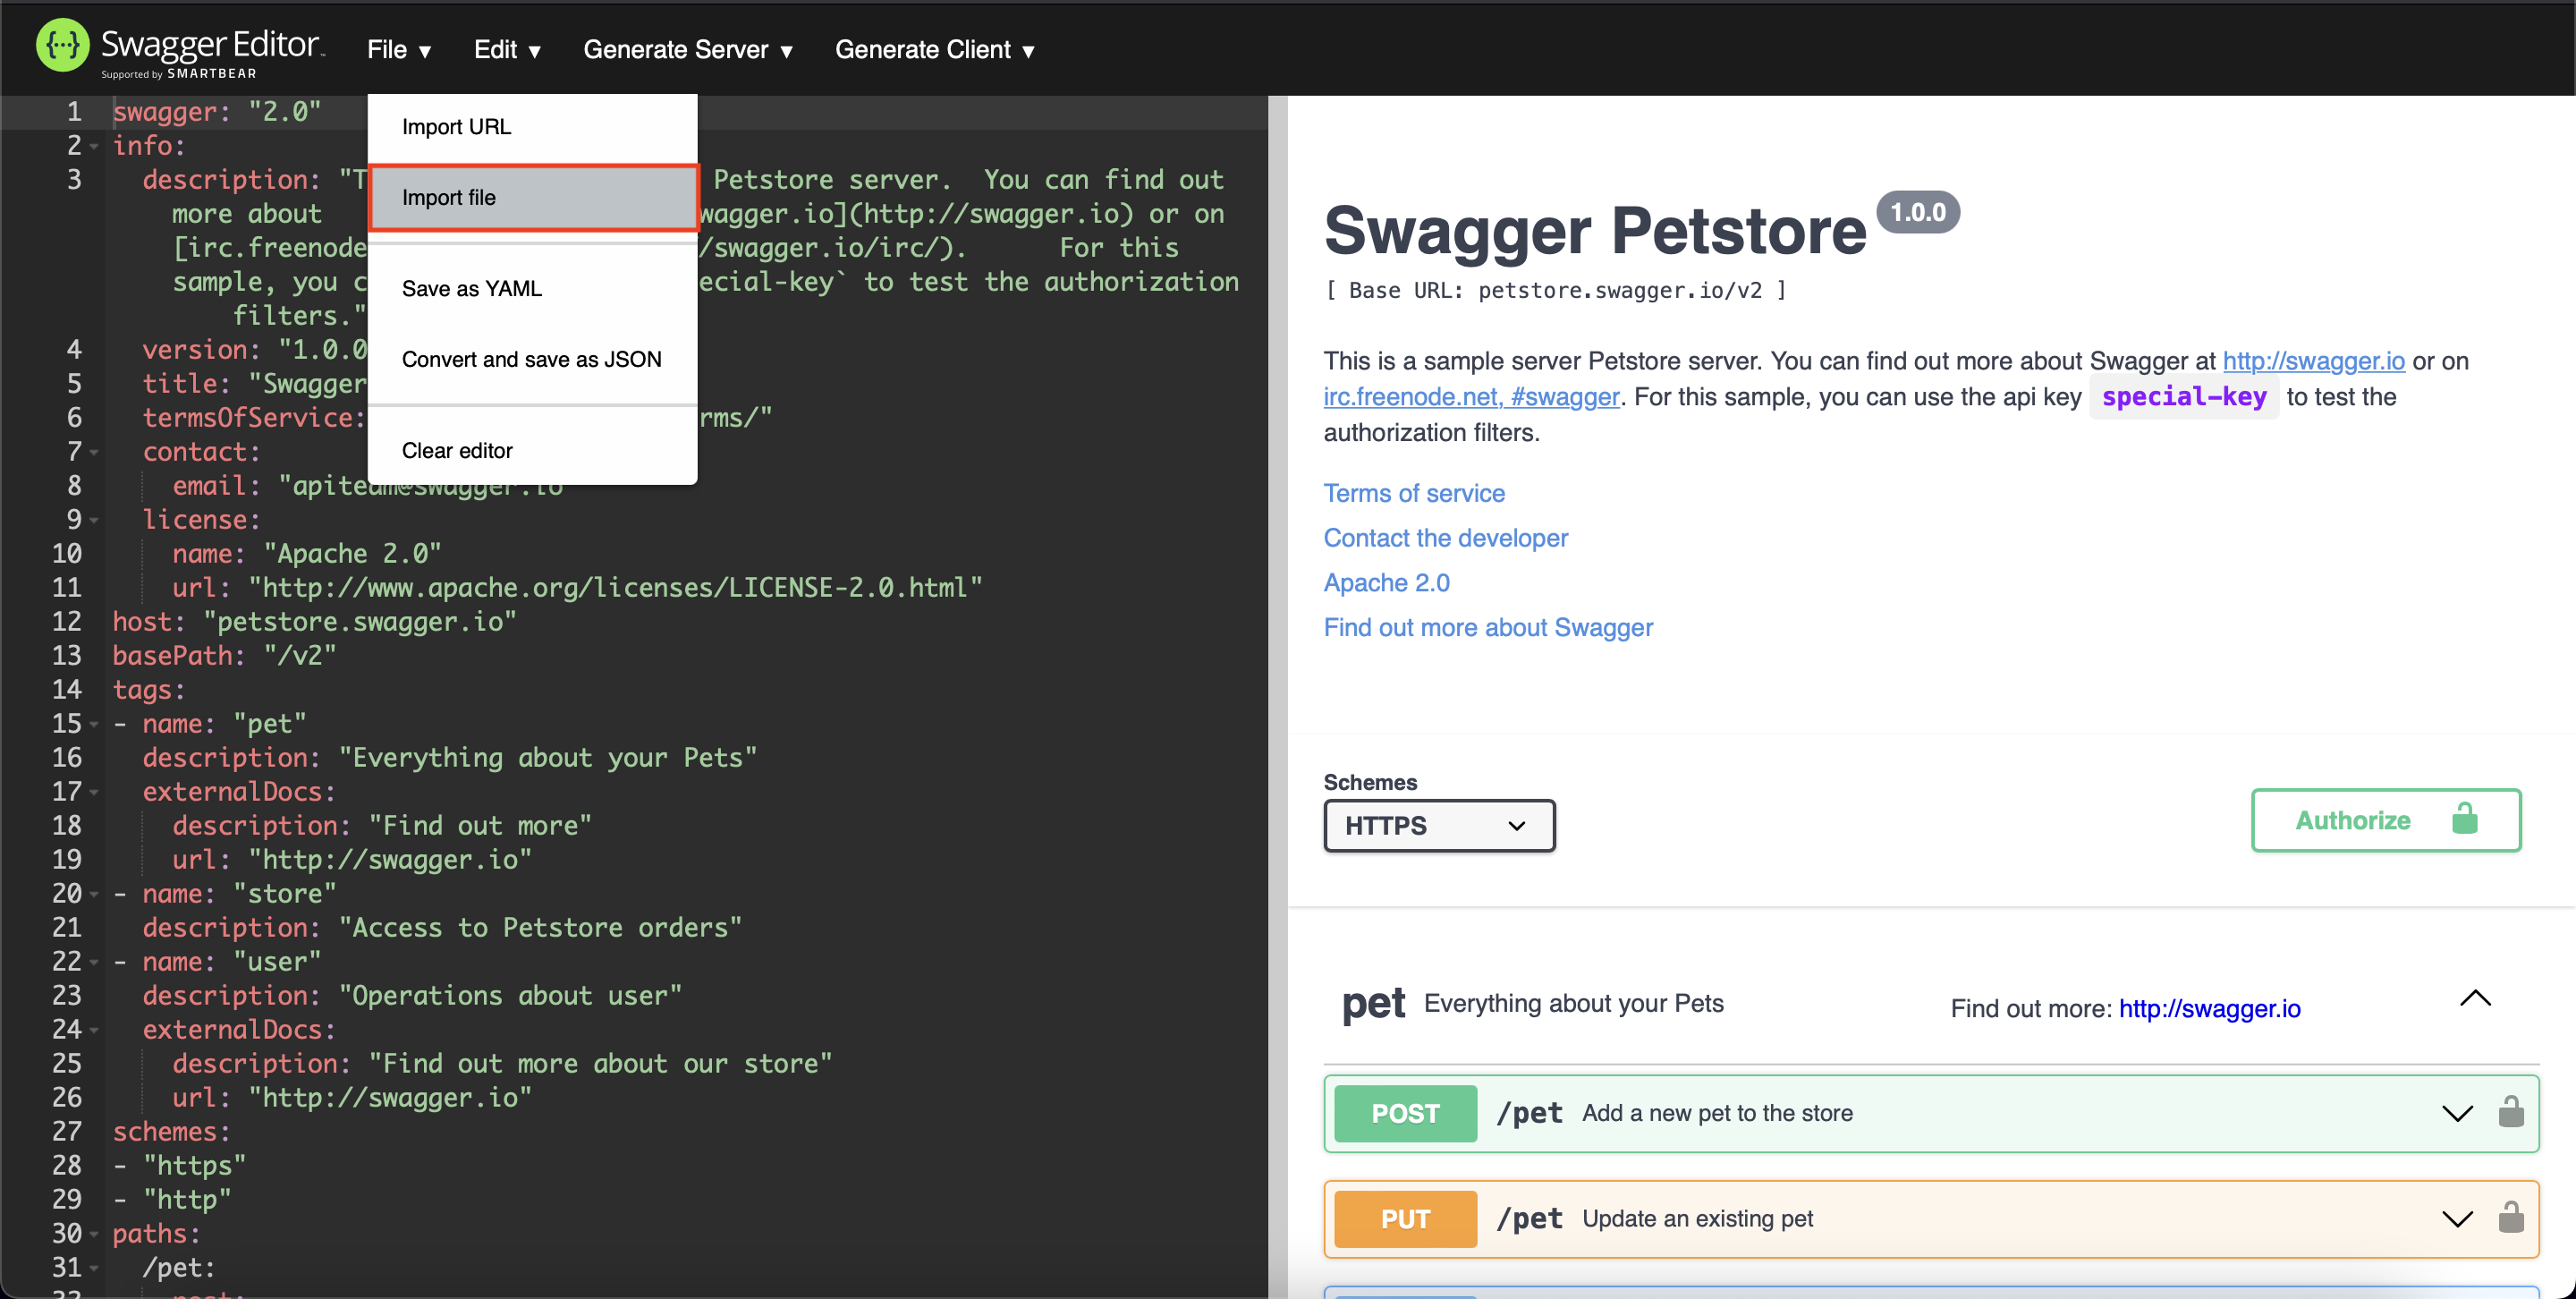
\includegraphics[width=\textwidth]{images/A-navrh-api/A-1-swagger-import.png}
    \caption{Vložení souboru do editoru Swagger}
\end{figure}

\begin{figure}
    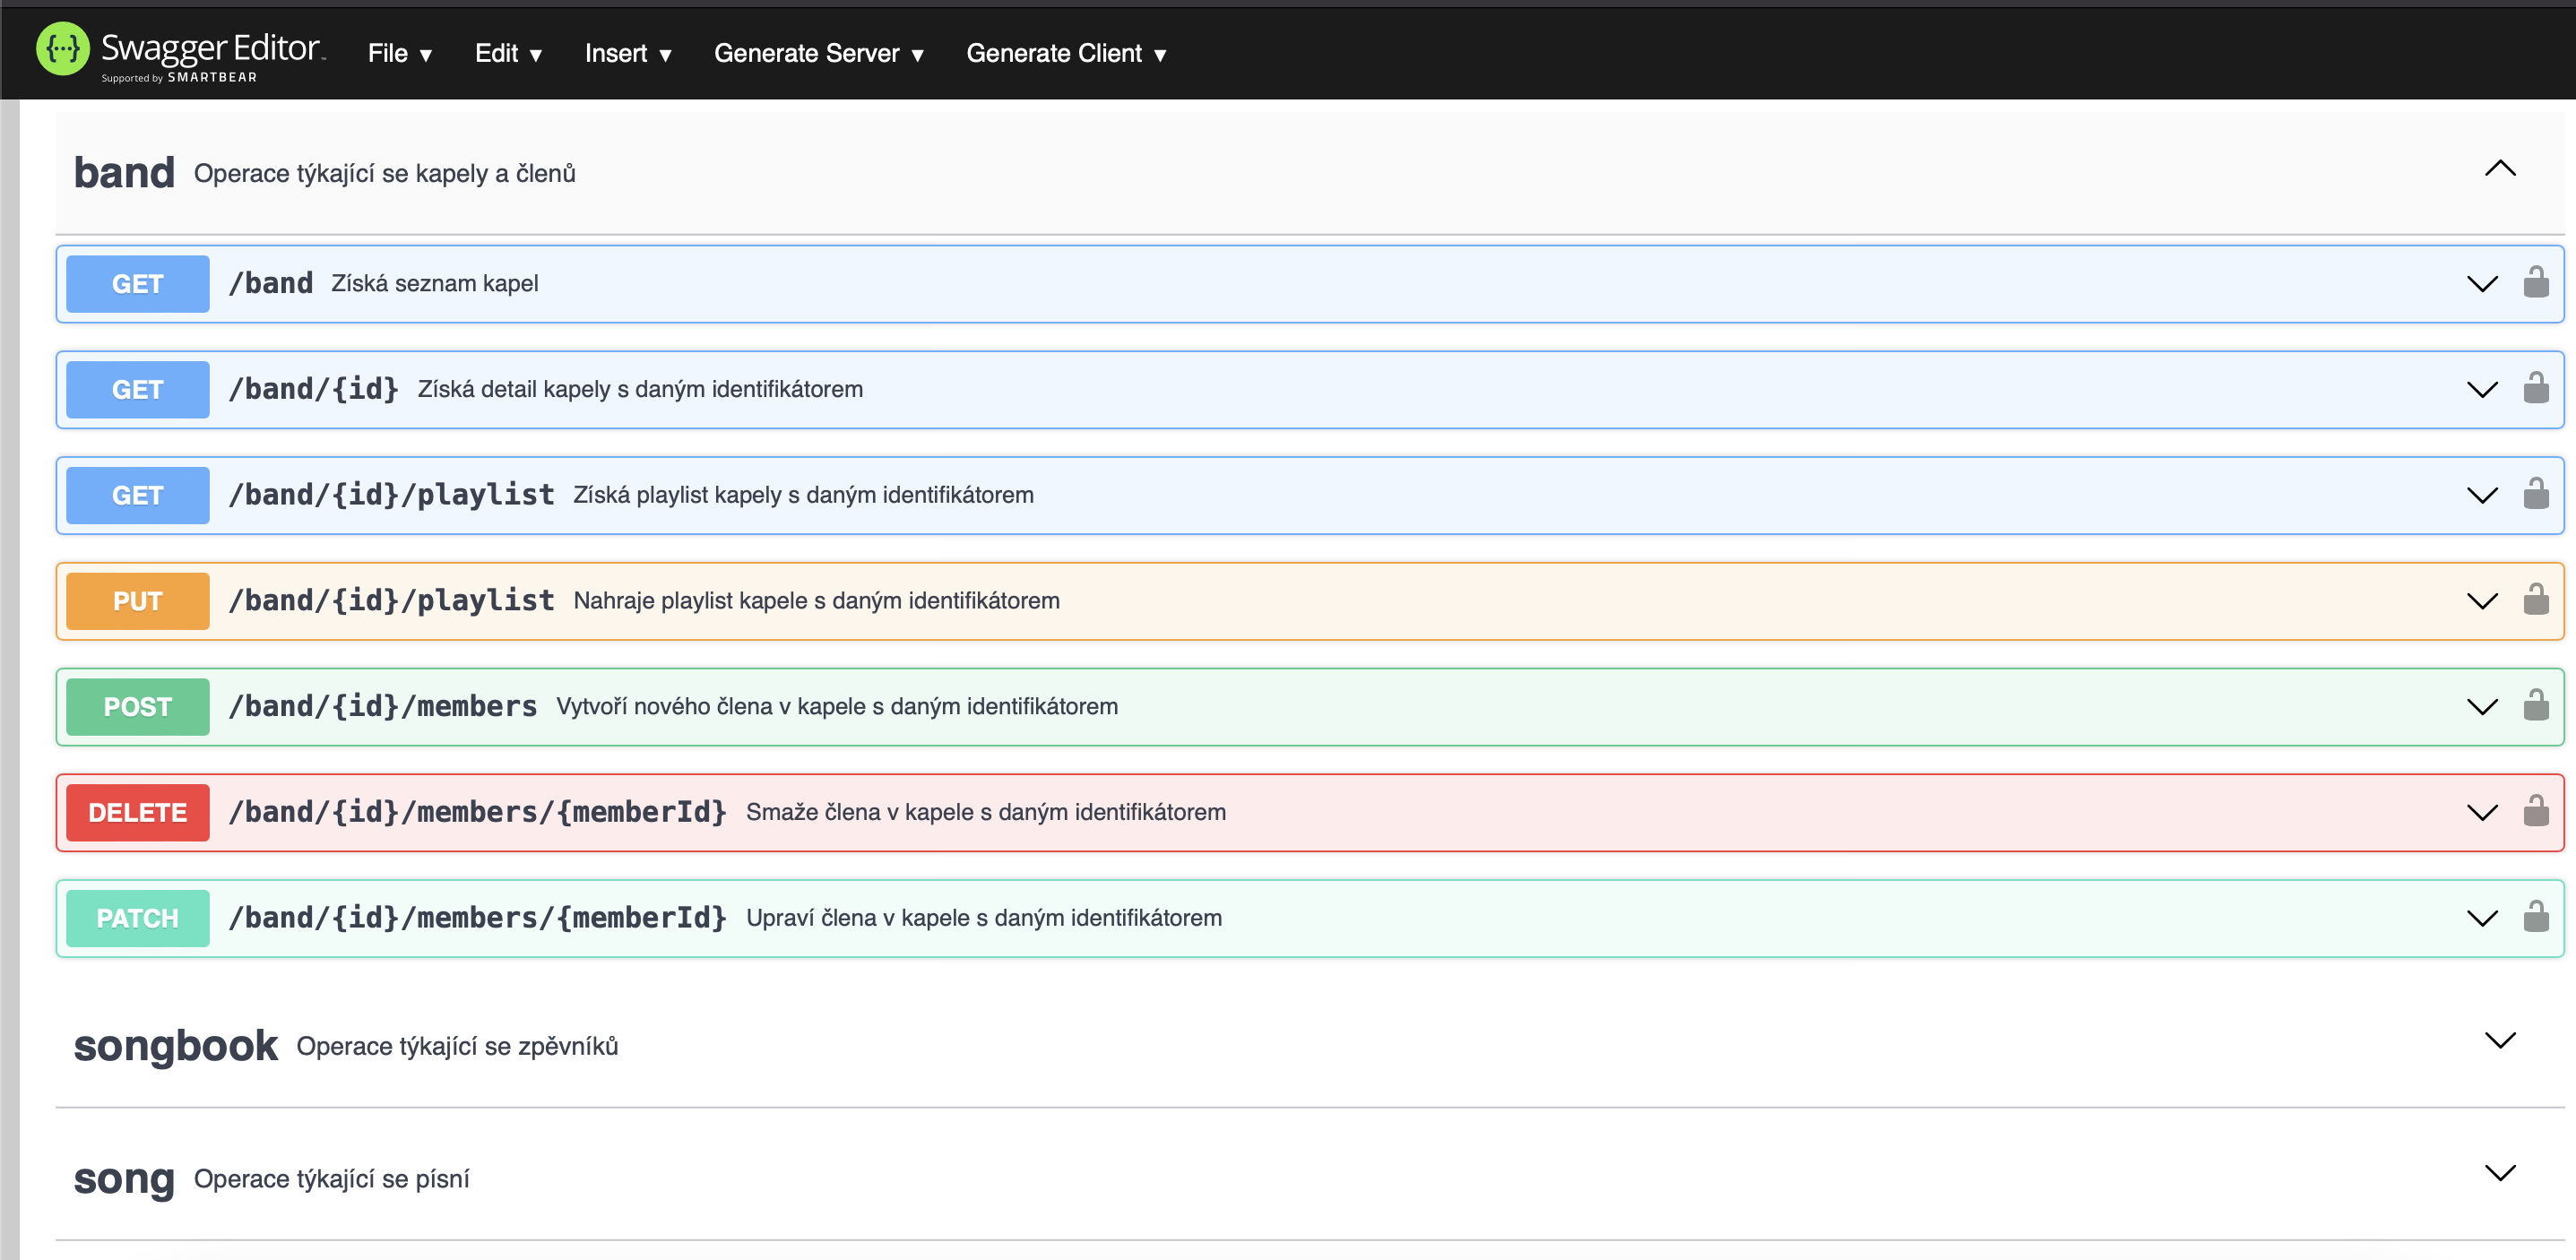
\includegraphics[width=\textwidth]{images/A-navrh-api/A-2-swagger-dokumentace.png}
    \caption{Ukázka vygenerované interaktivní dokumentace v editoru Swagger}
\end{figure}

\begin{figure}
    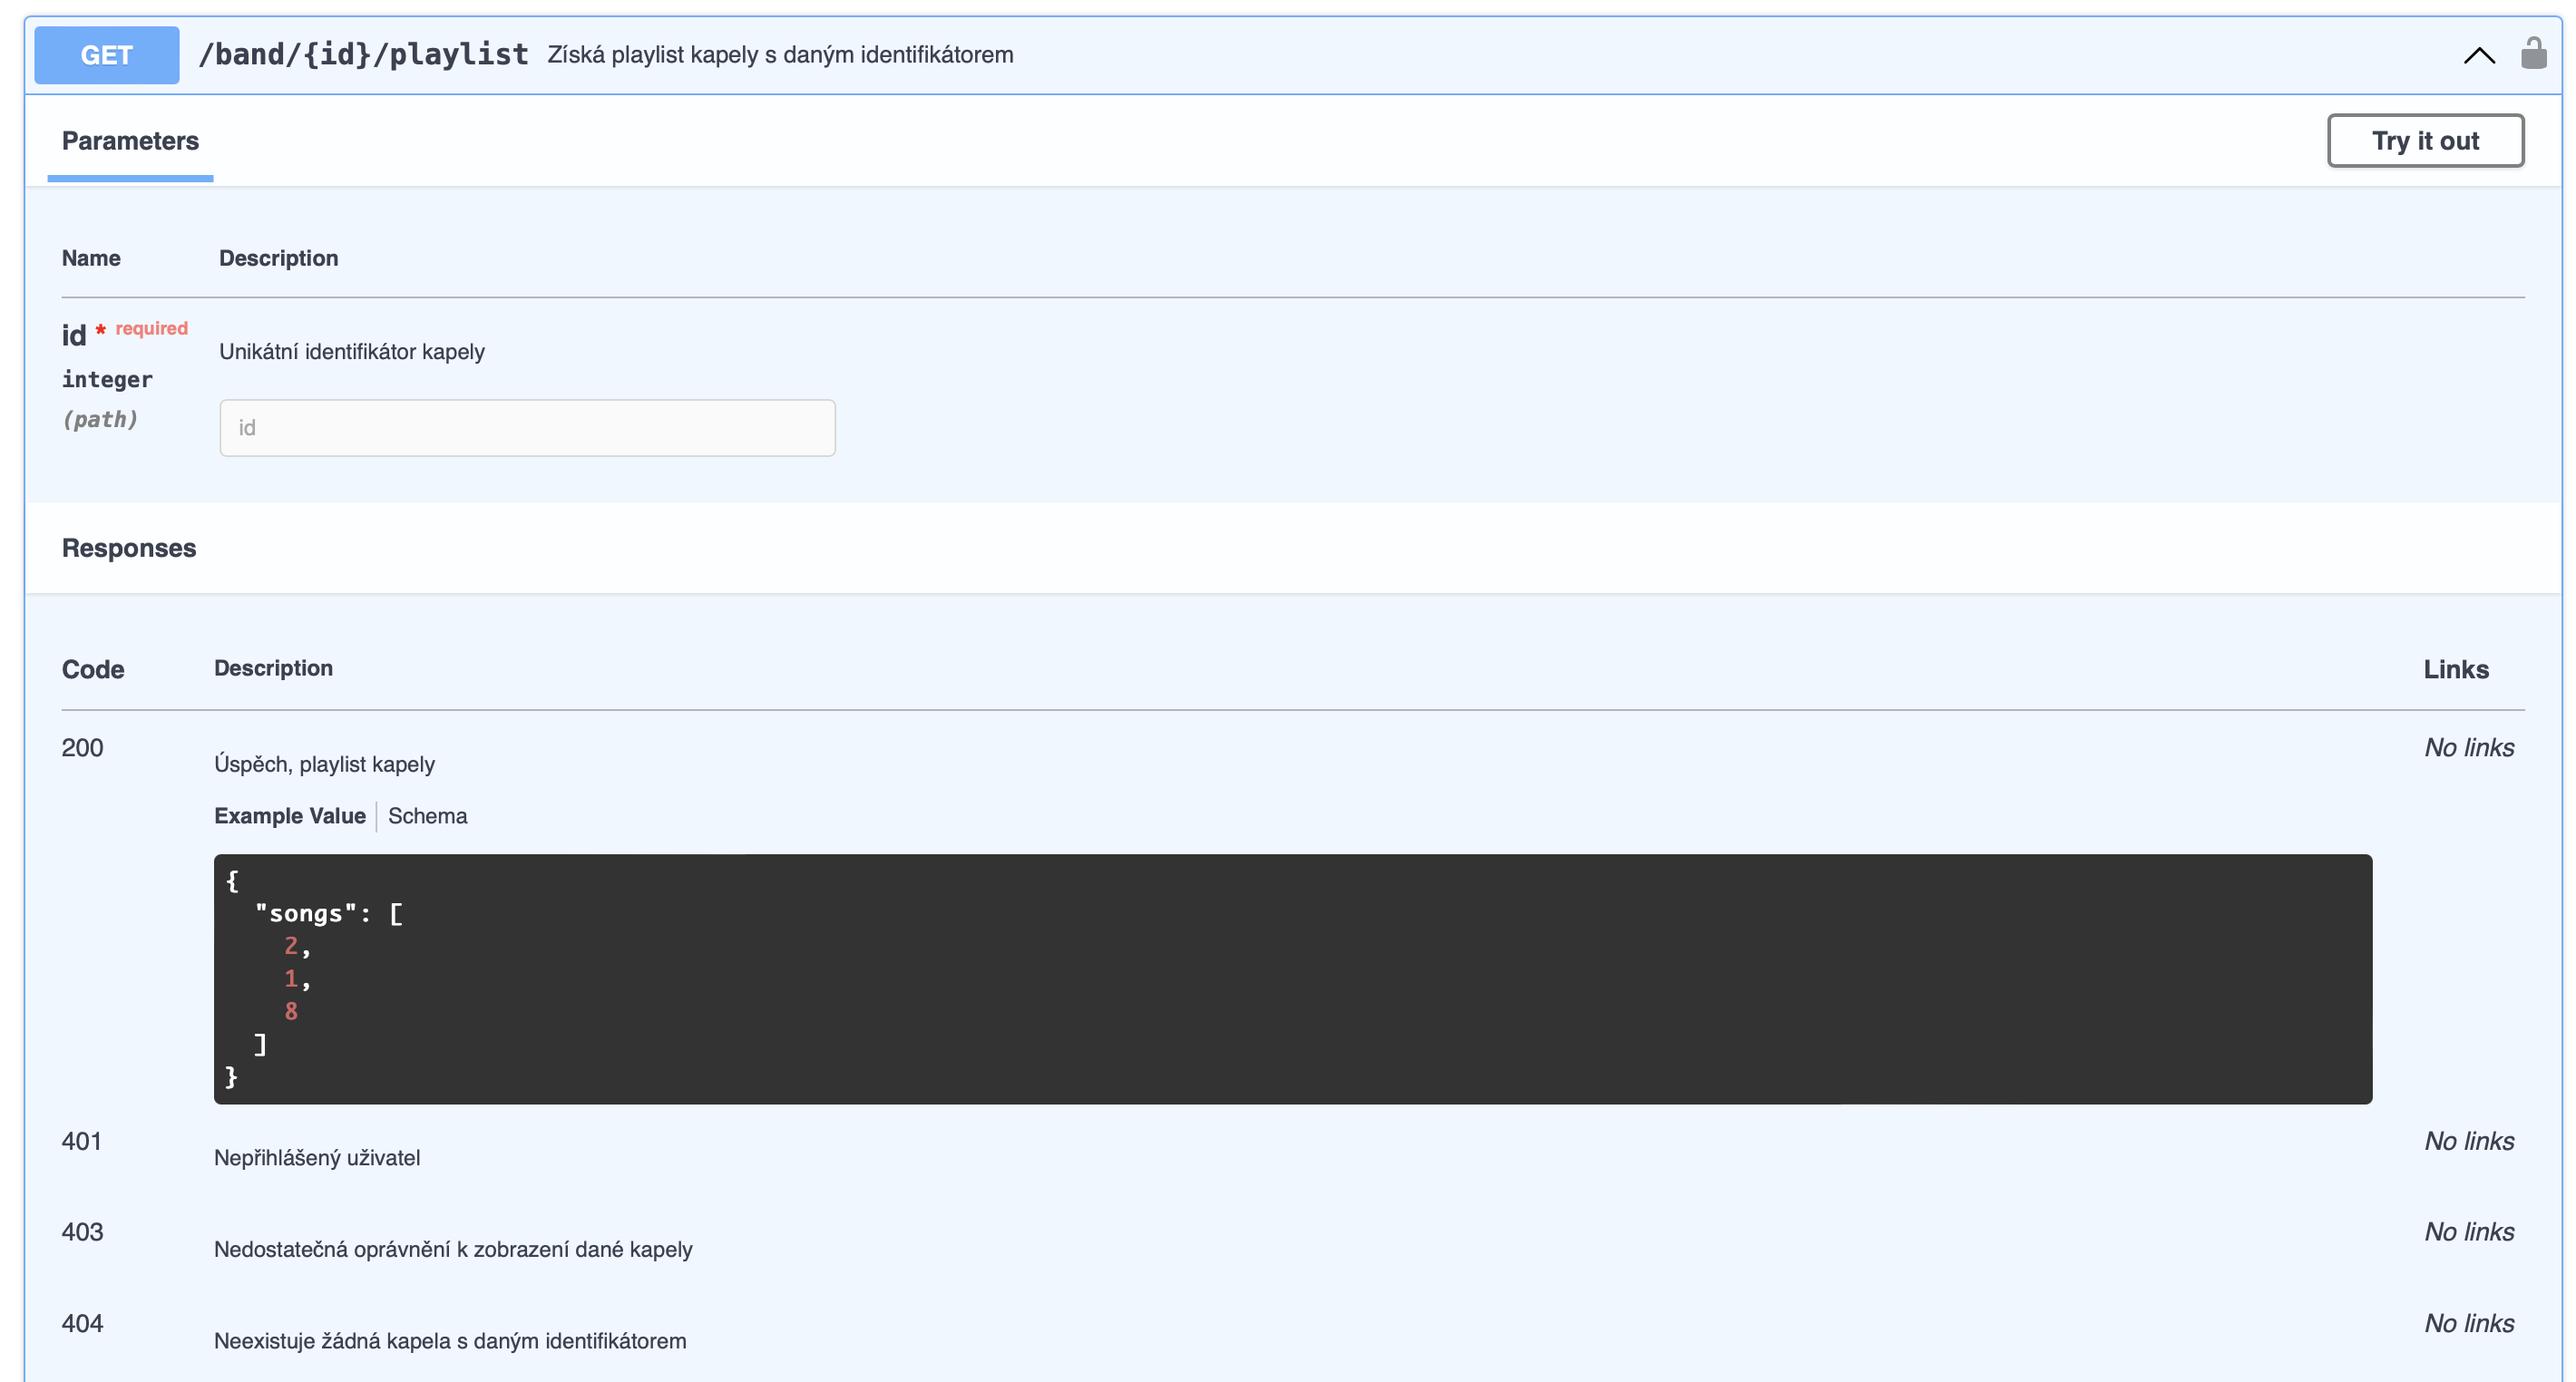
\includegraphics[width=\textwidth]{images/A-navrh-api/A-3-swagger-dokumentace-detail.png}
    \caption{Detail vygenerované dokumentace v editoru Swagger}
\end{figure}

\chapter{Návrh uživatelského rozhraní}

\begin{figure}[H]
    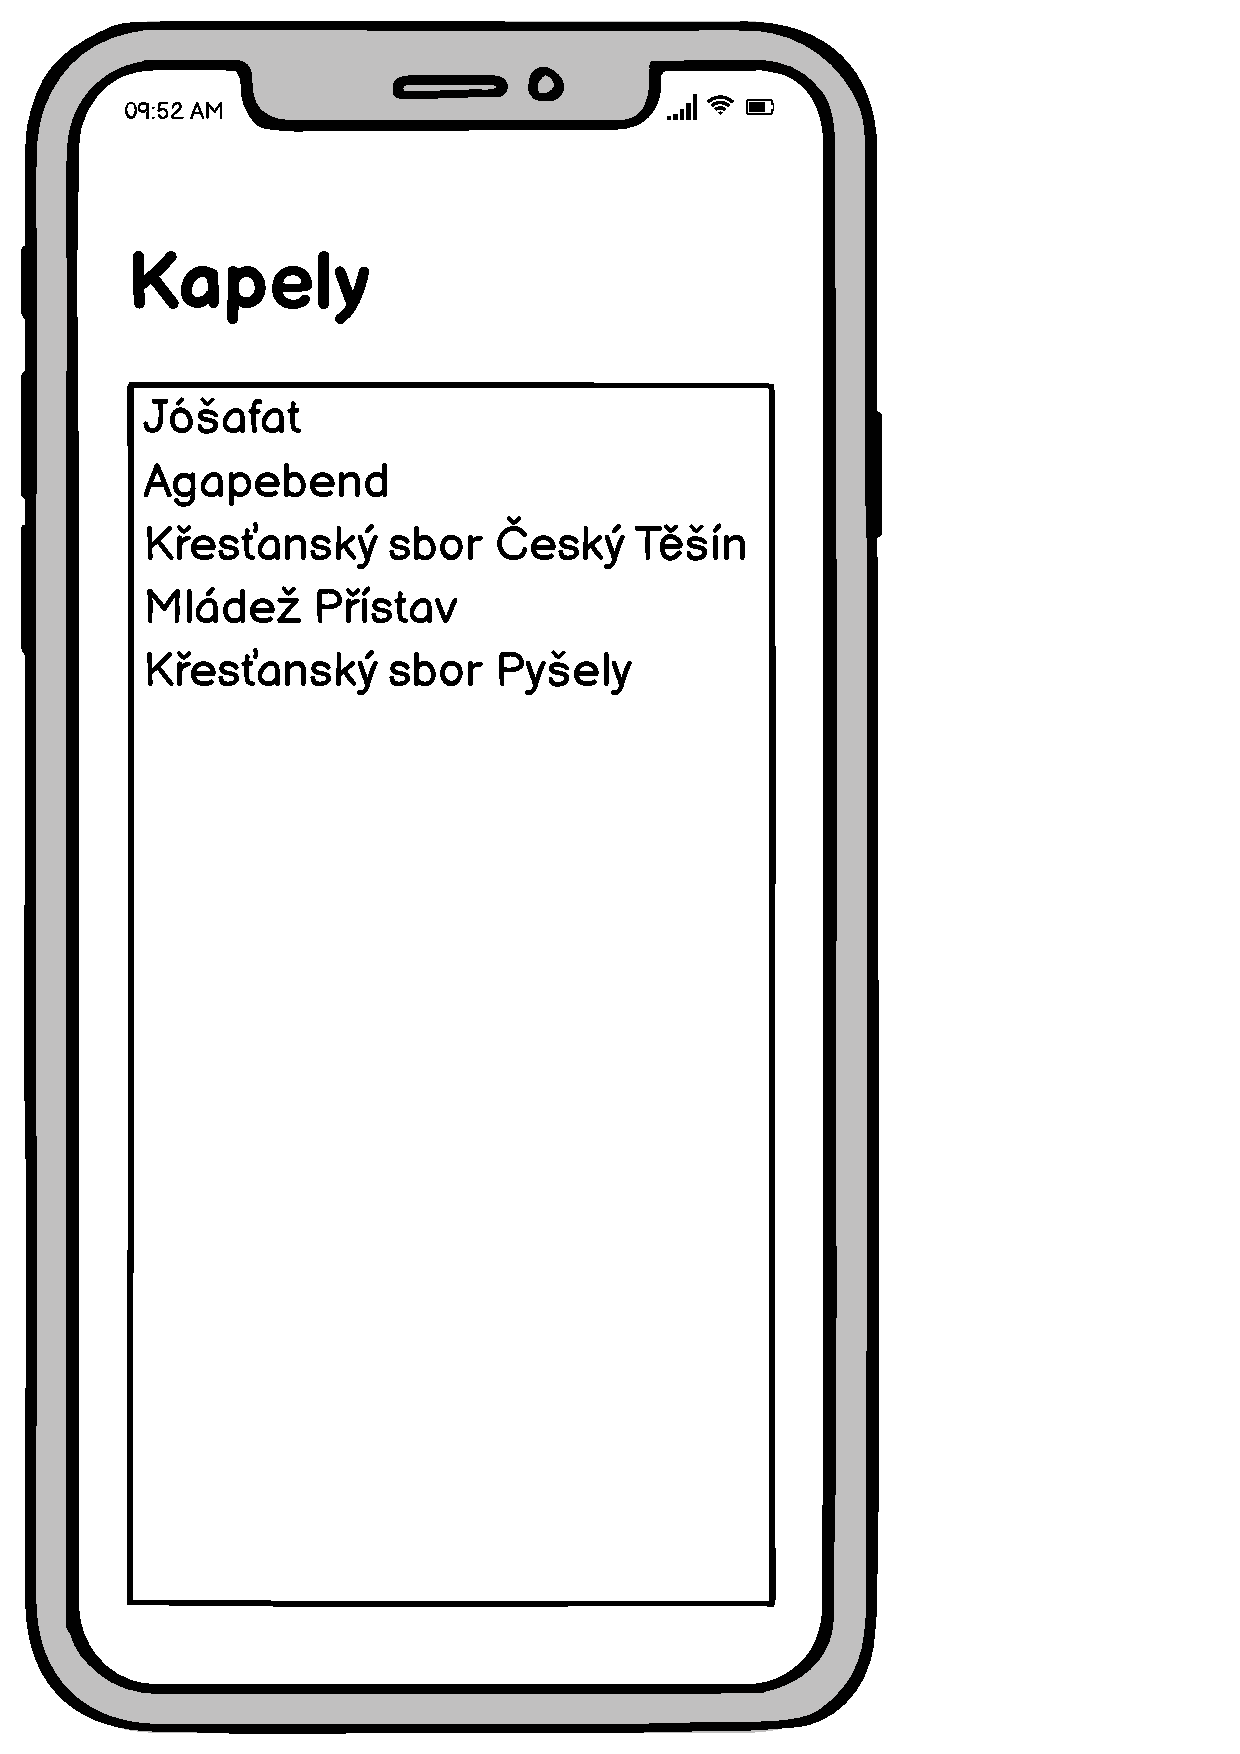
\includegraphics[width=0.45\textwidth]{images/B-navrh-ui/B-1-vyber-kapely.pdf}
    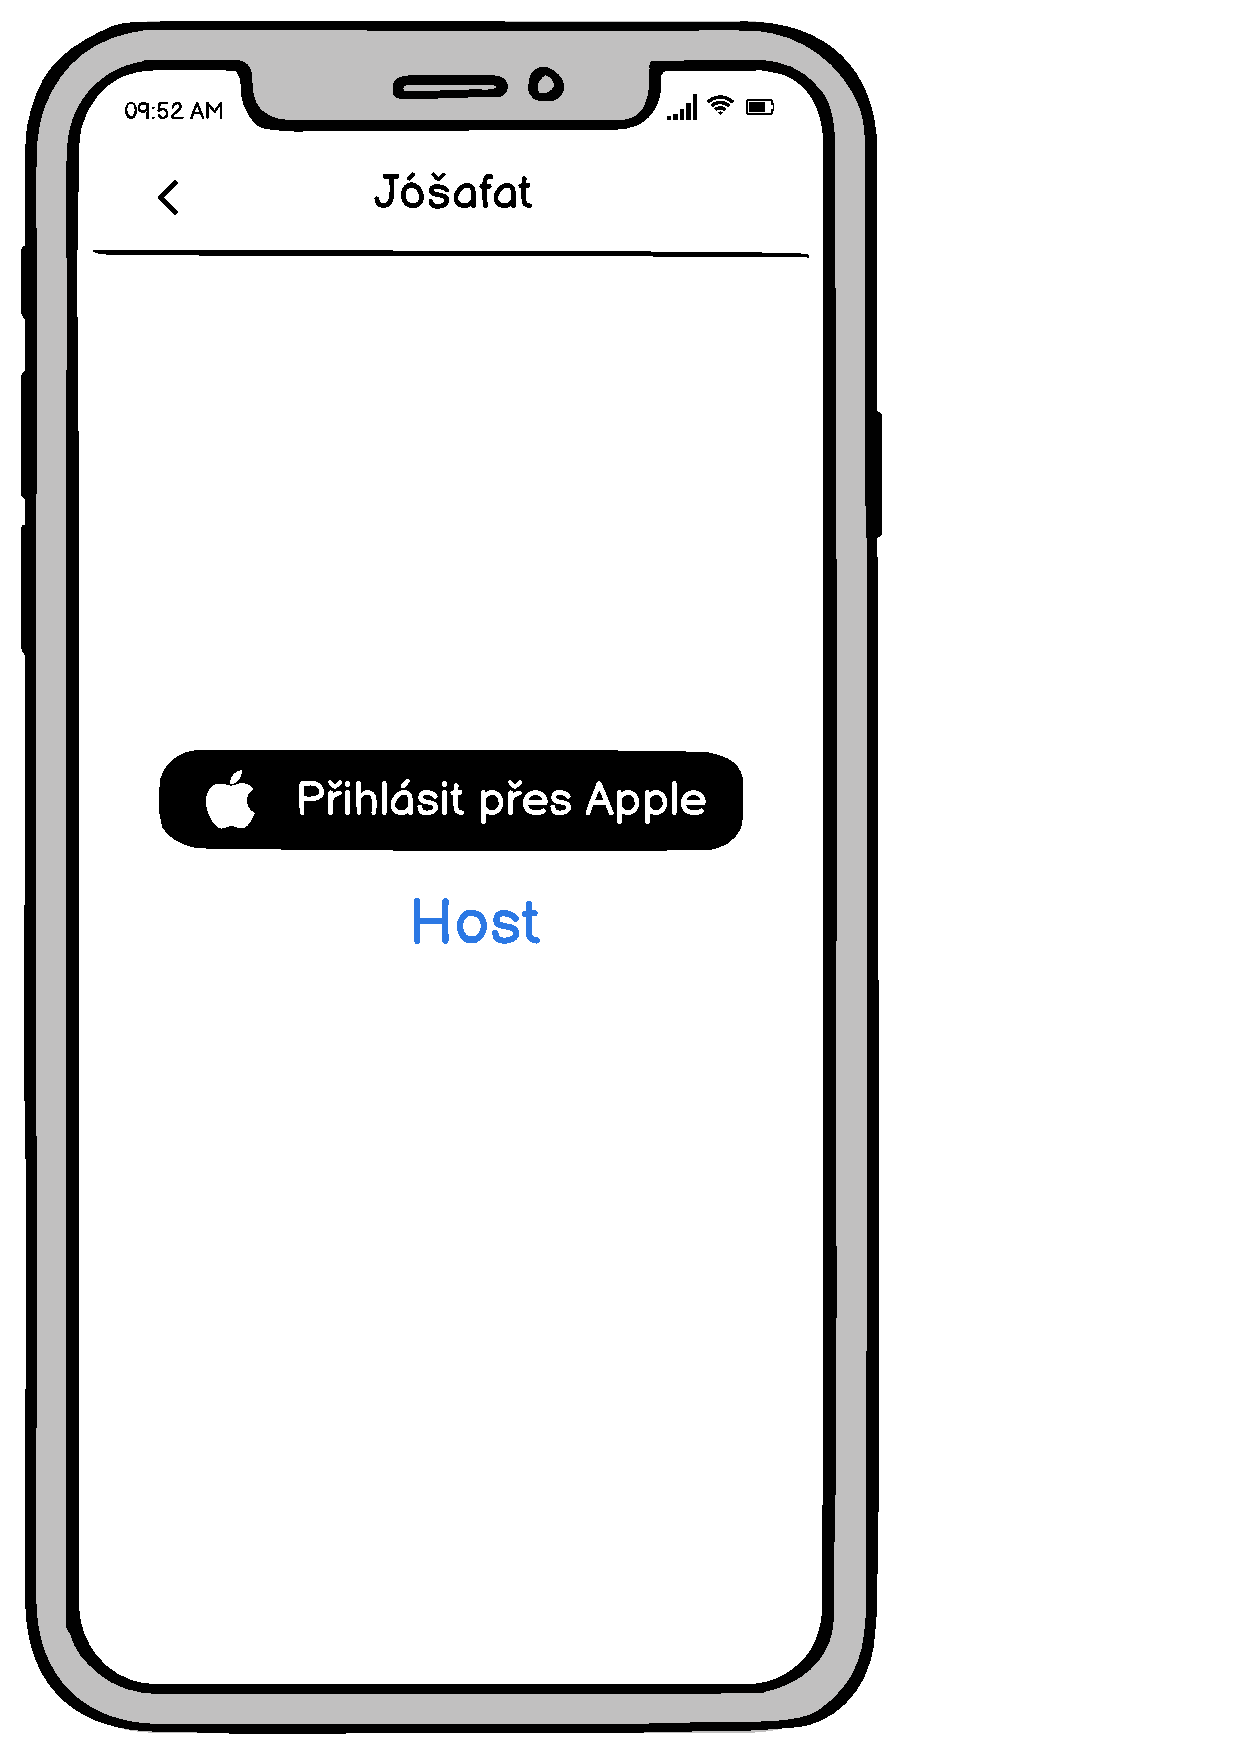
\includegraphics[width=0.45\textwidth]{images/B-navrh-ui/B-1-prihlaseni.pdf}
    \caption{Výběr kapely a Přihlášení}
\end{figure}

% Stránka 2

\begin{figure}
    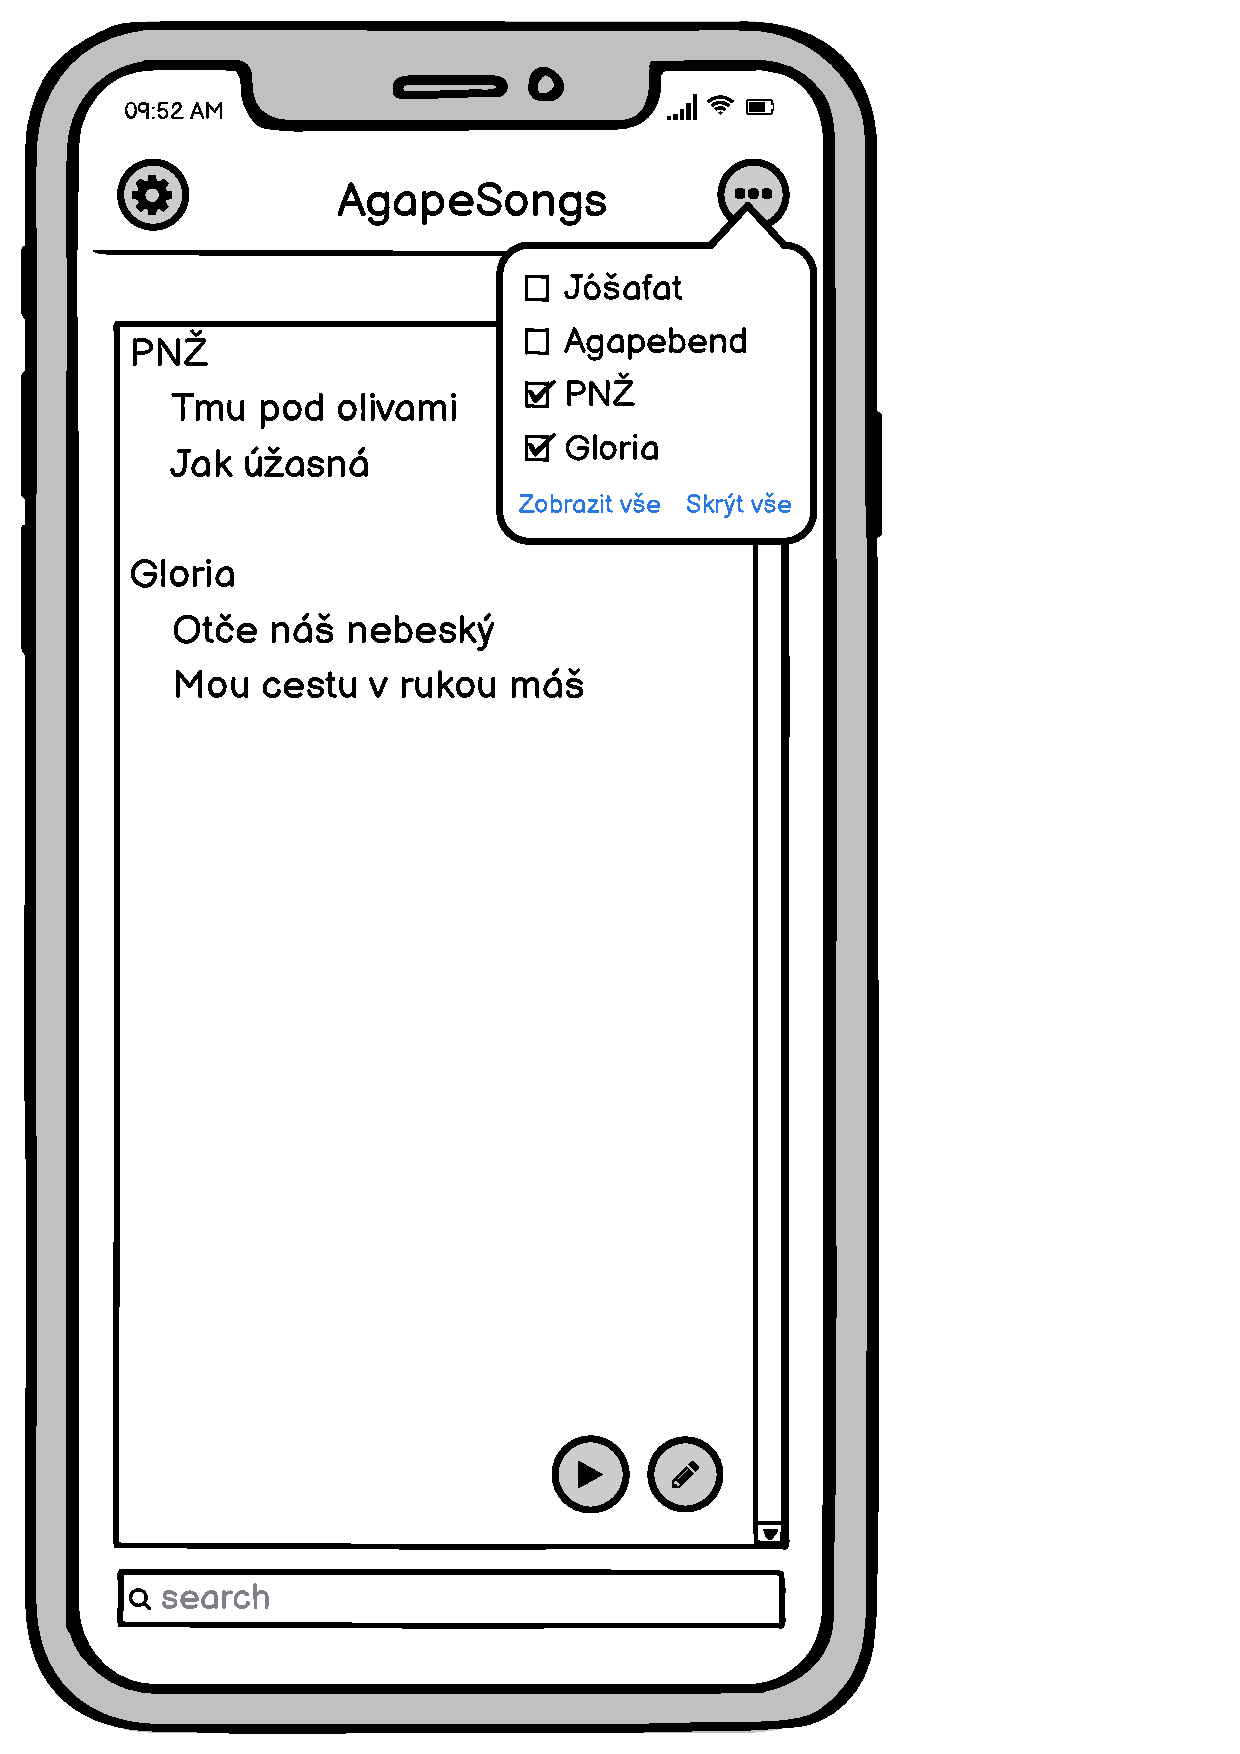
\includegraphics[width=0.49\textwidth]{images/B-navrh-ui/B-2-seznam-pisni.pdf}
    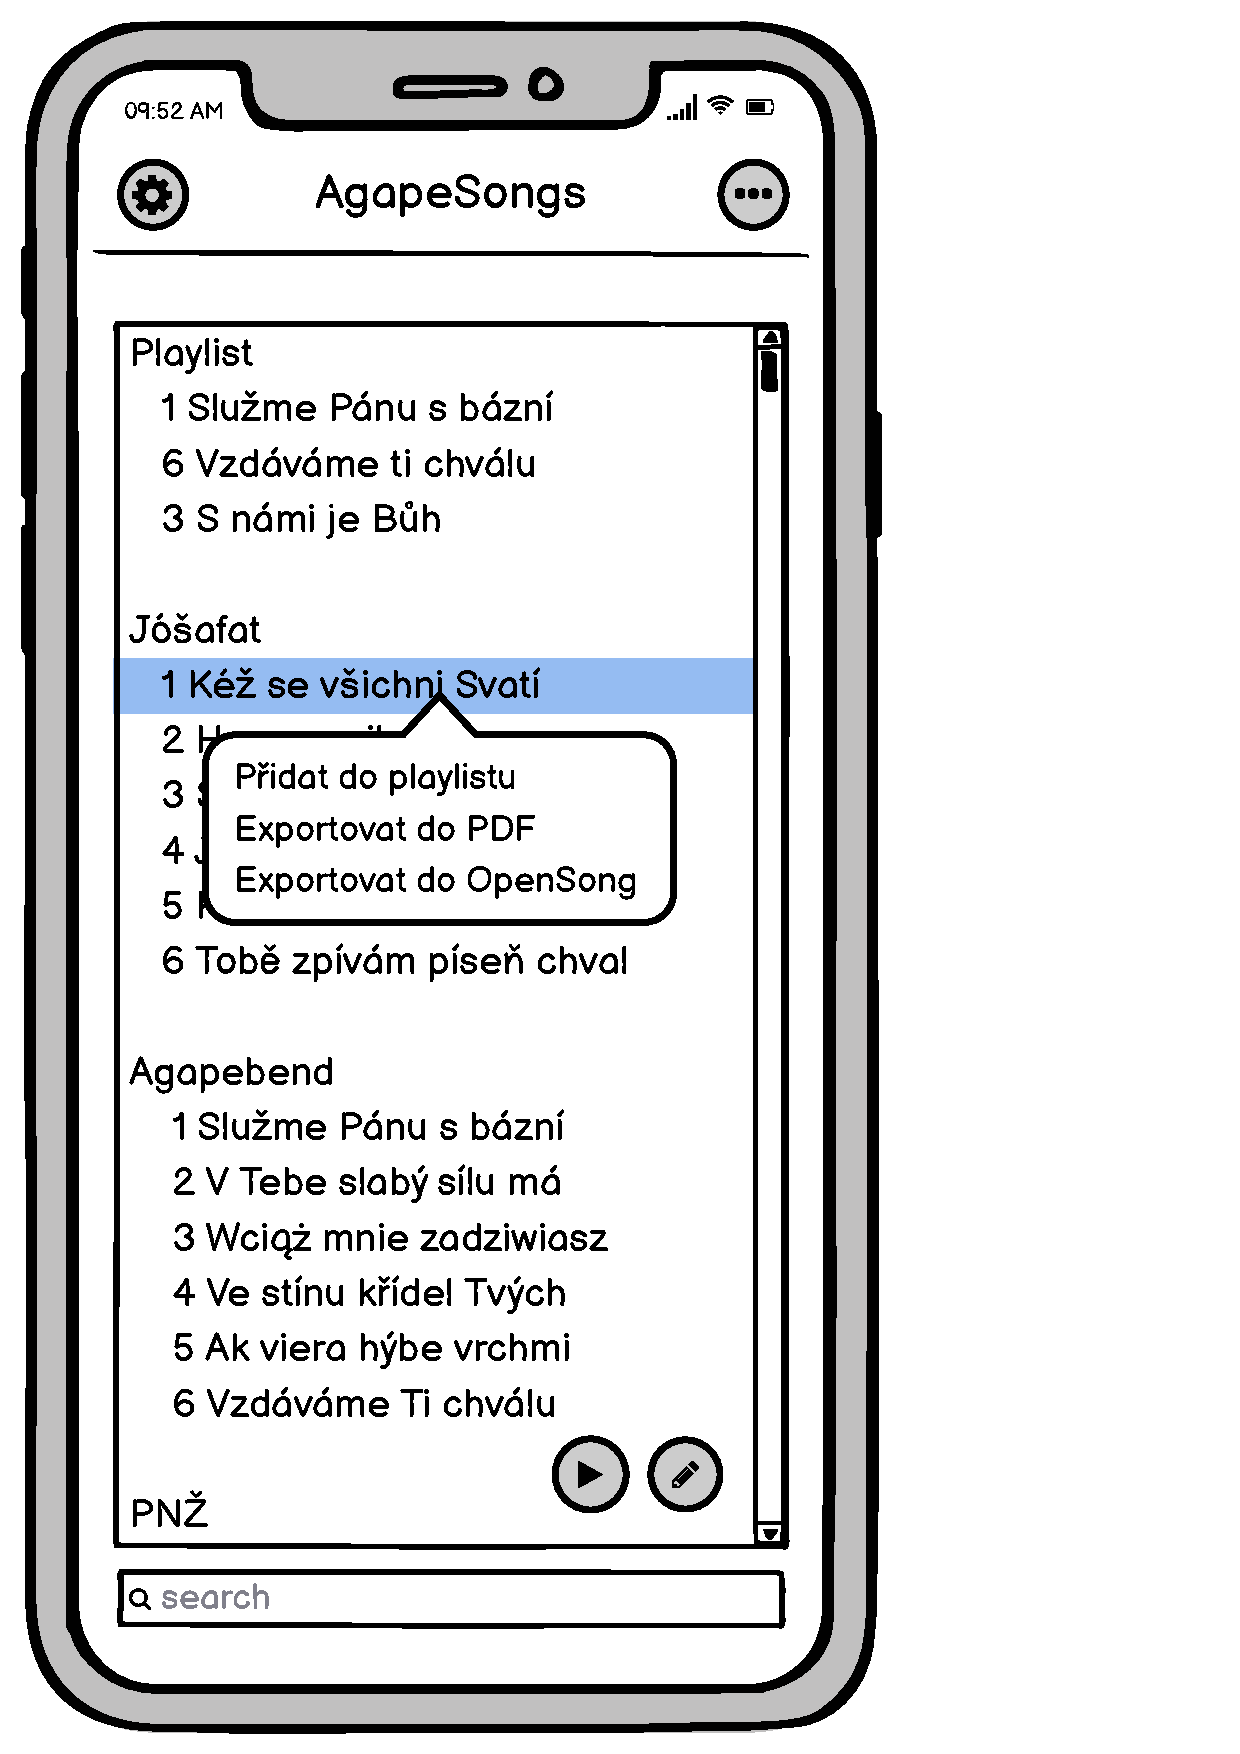
\includegraphics[width=0.49\textwidth]{images/B-navrh-ui/B-2-seznam-pisni-kontextove-menu.pdf}
    \caption{Seznam písní a kontextové menu pro přidání písně do playlistu a export písně}
\end{figure}

% Stránka 3

\begin{figure}
    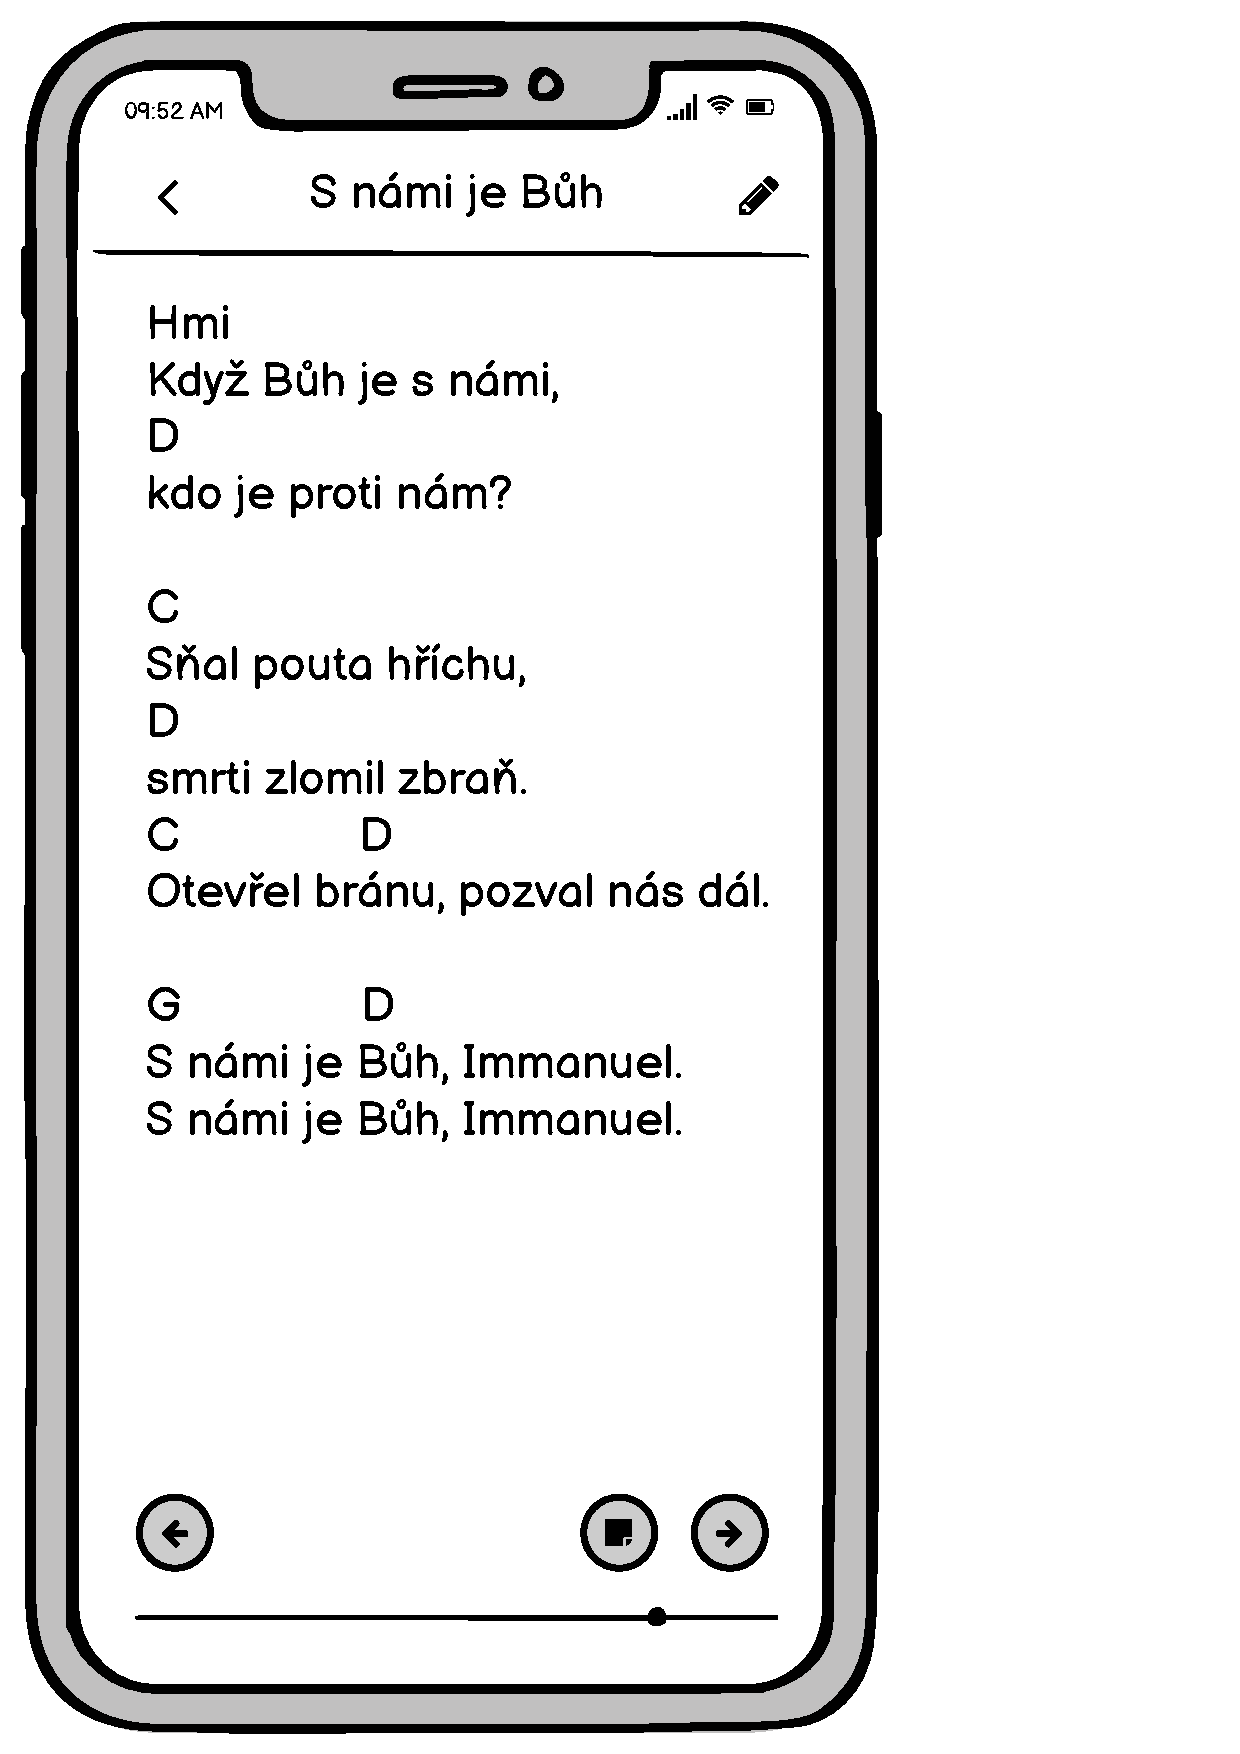
\includegraphics[width=0.49\textwidth]{images/B-navrh-ui/B-3-detail-pisne.pdf}
    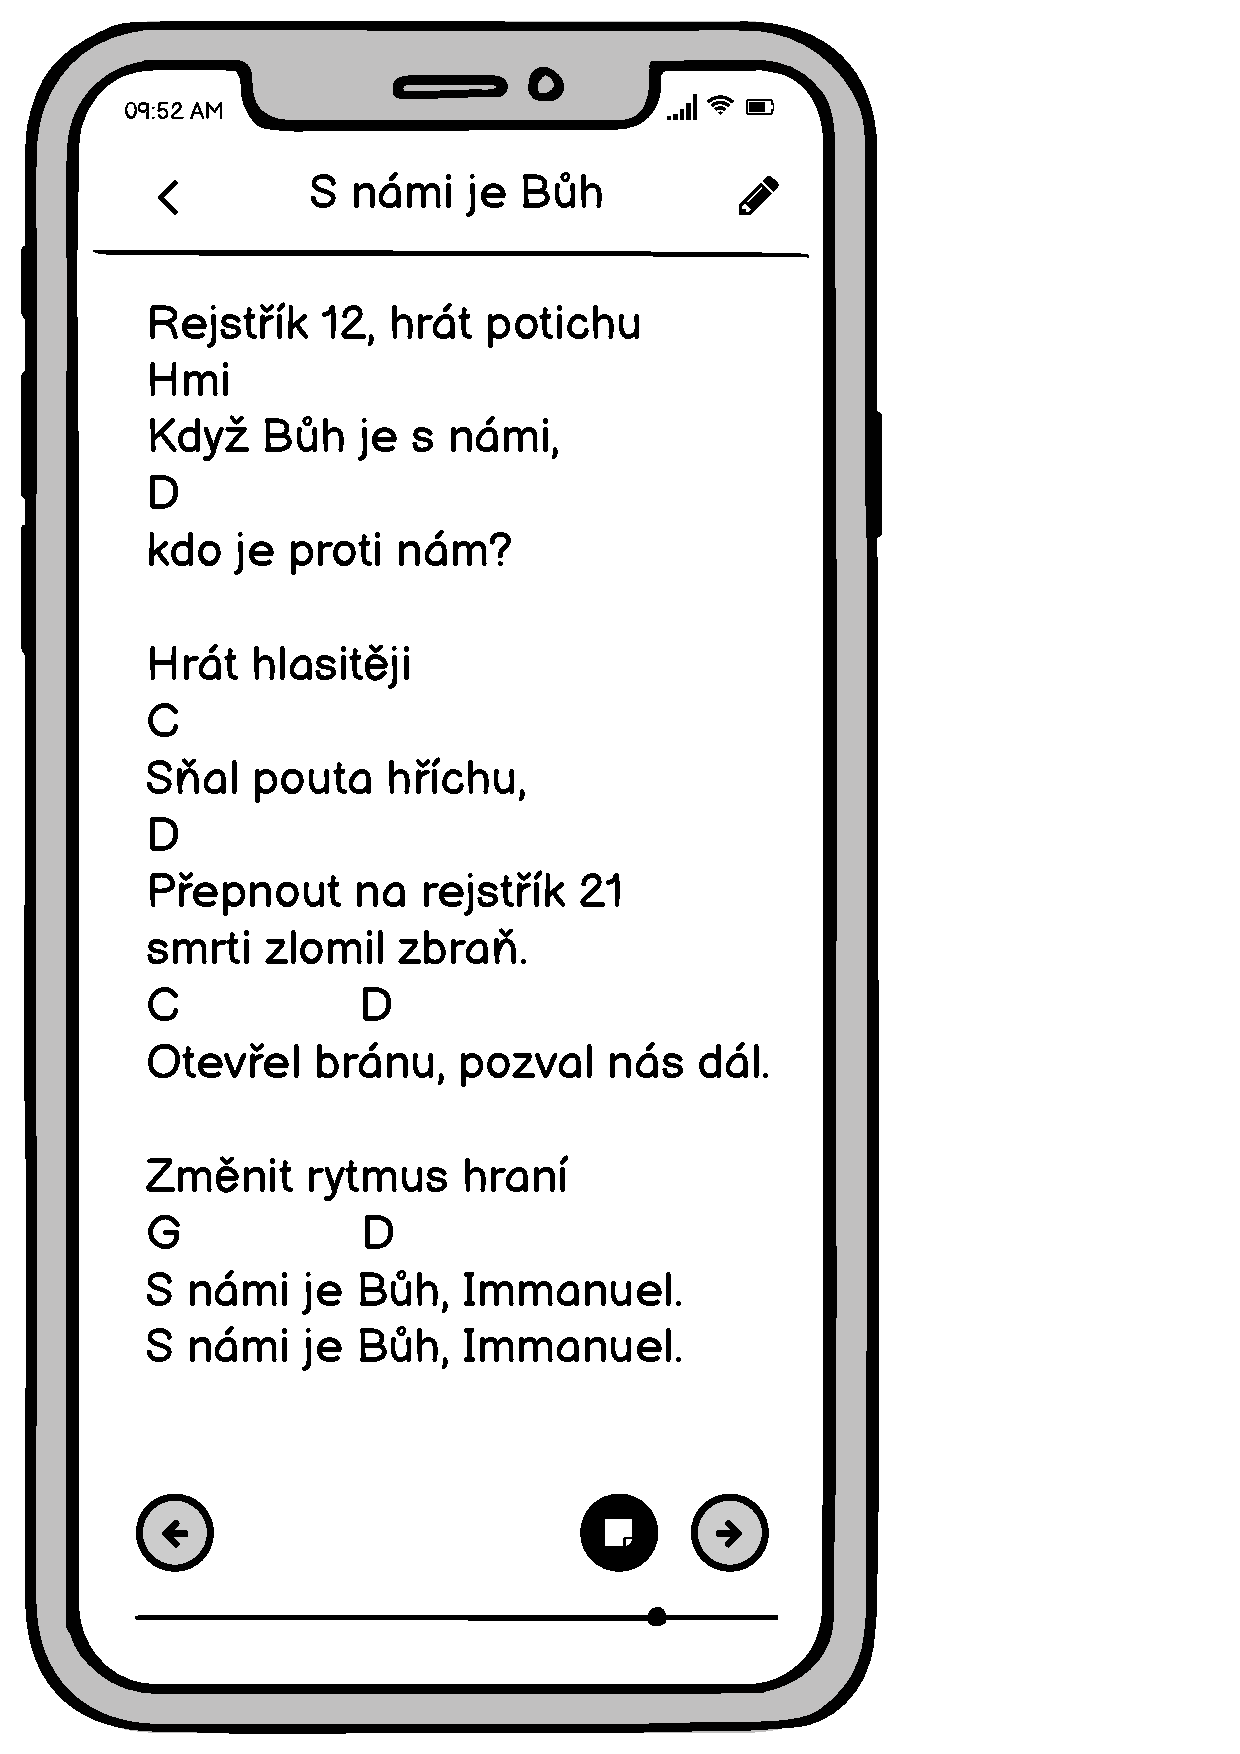
\includegraphics[width=0.49\textwidth]{images/B-navrh-ui/B-3-detail-pisne-poznamky.pdf}
    \caption{Detail písně bez a se zapnutými poznámkami}
\end{figure}

% Stránka 4

\begin{figure}
    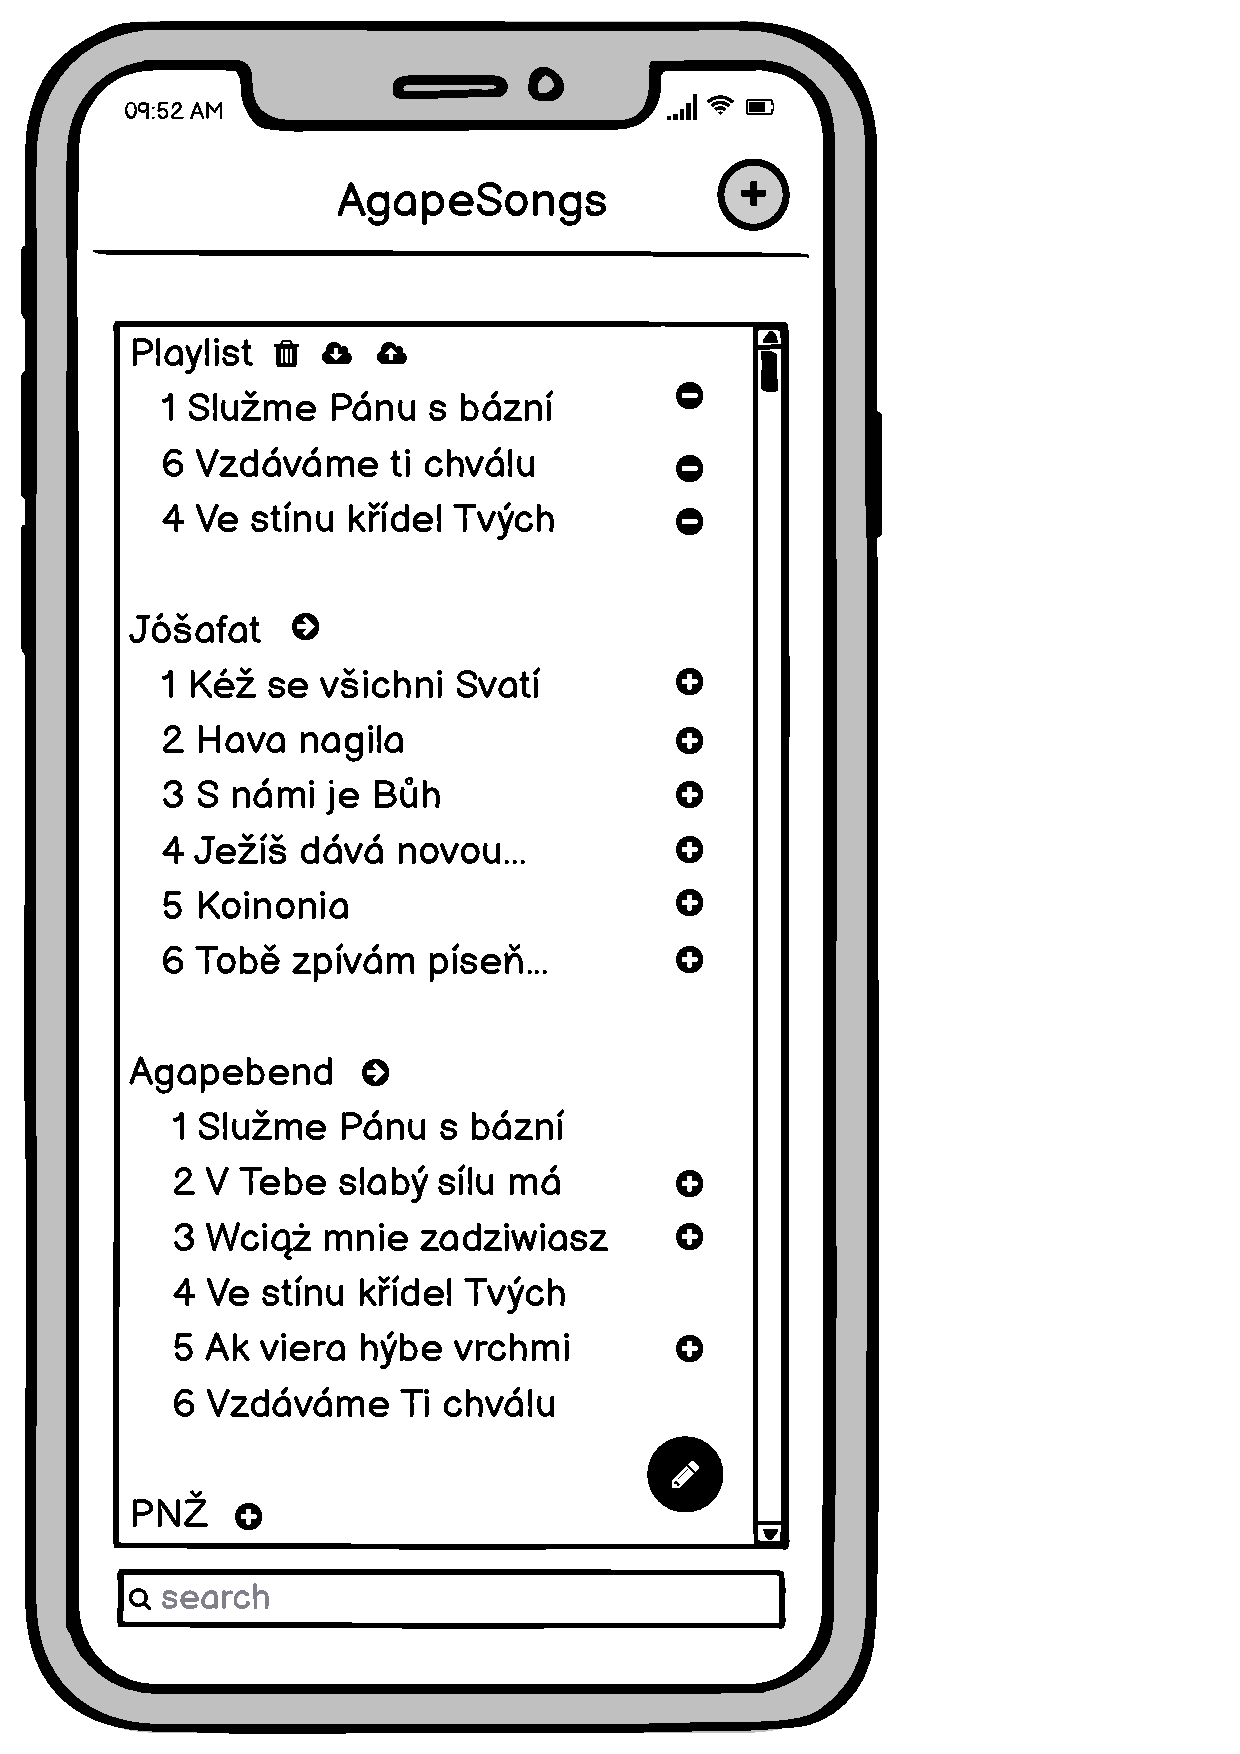
\includegraphics[width=0.49\textwidth]{images/B-navrh-ui/B-4-sprava-playlistu-zpevniku.pdf}
    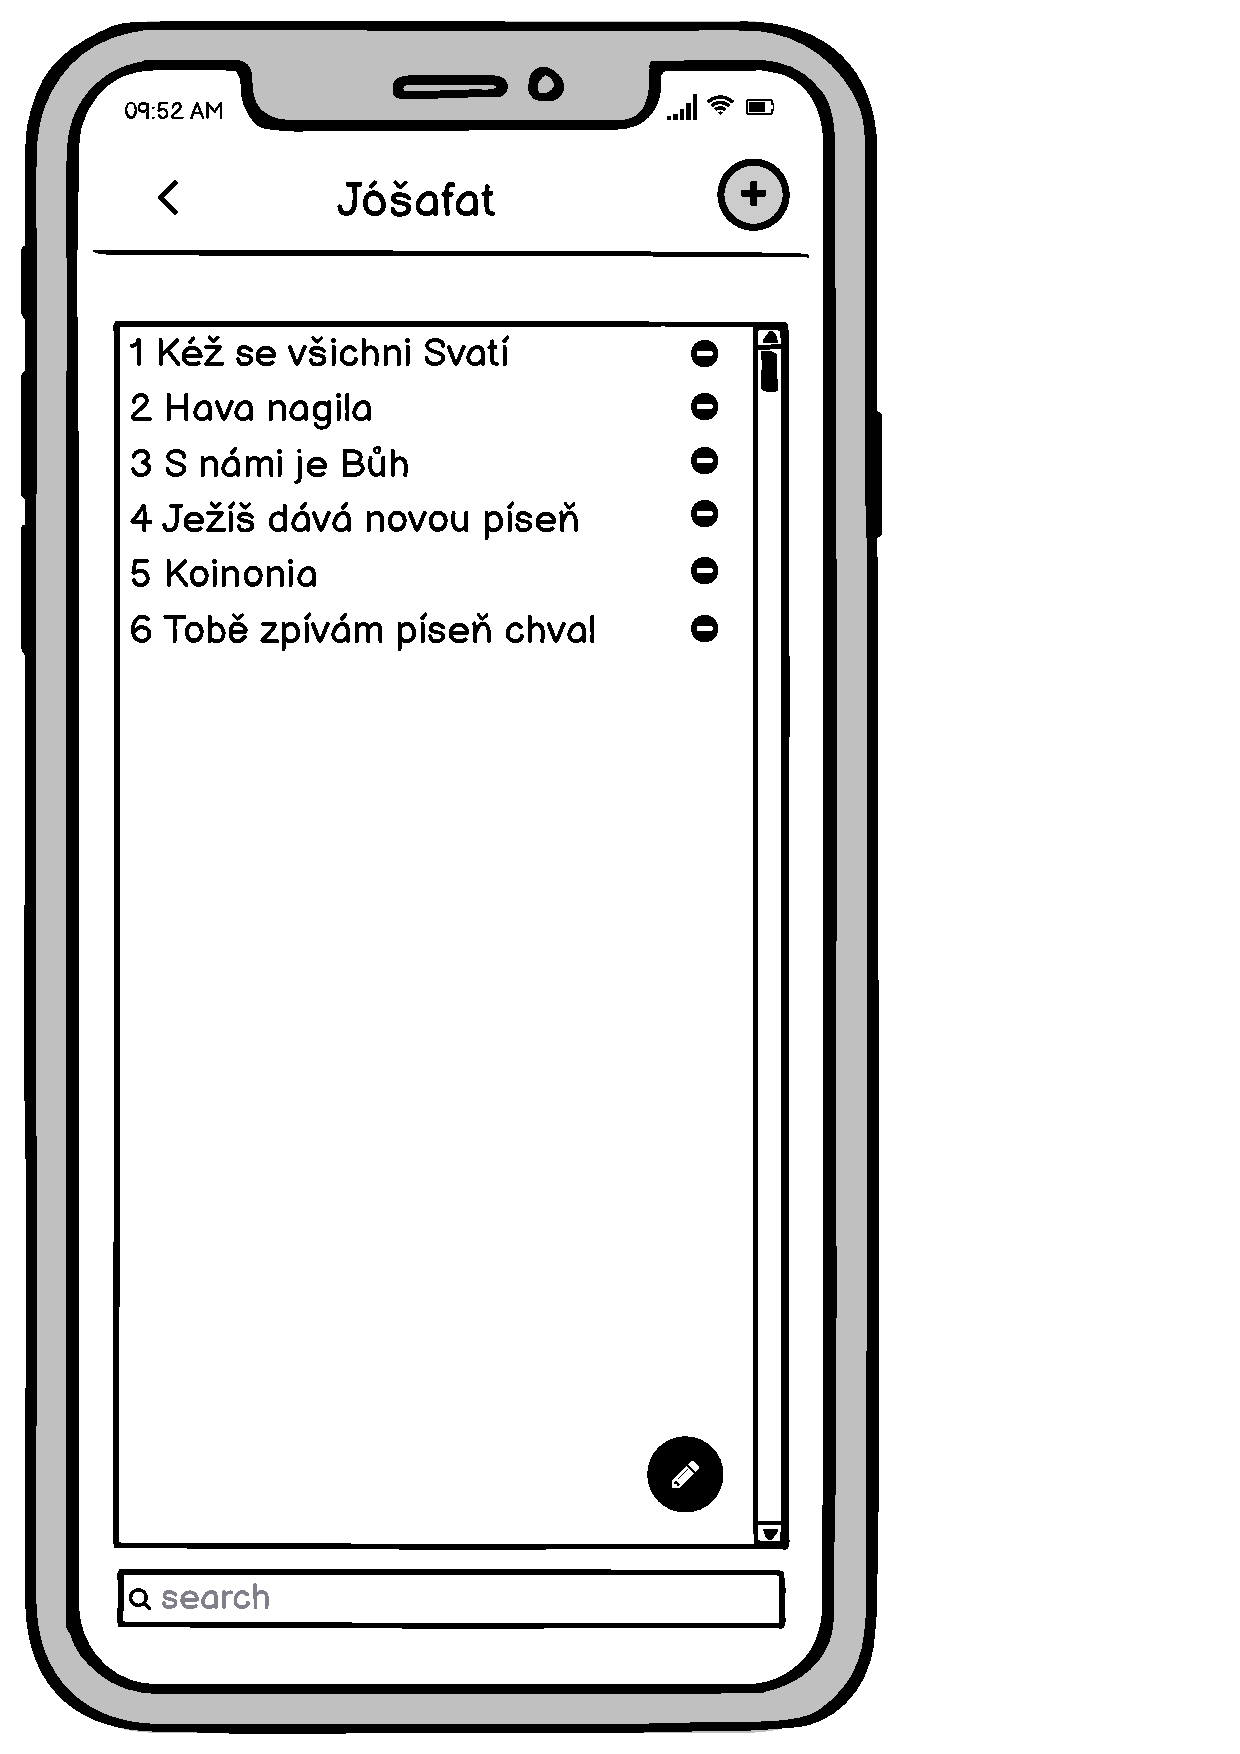
\includegraphics[width=0.49\textwidth]{images/B-navrh-ui/B-4-sprava-pisni.pdf}
    \caption{Správa playlistů, zpěvníků a Správa písní ve zpěvníku}
\end{figure}

% Stránka 5

\begin{figure}
    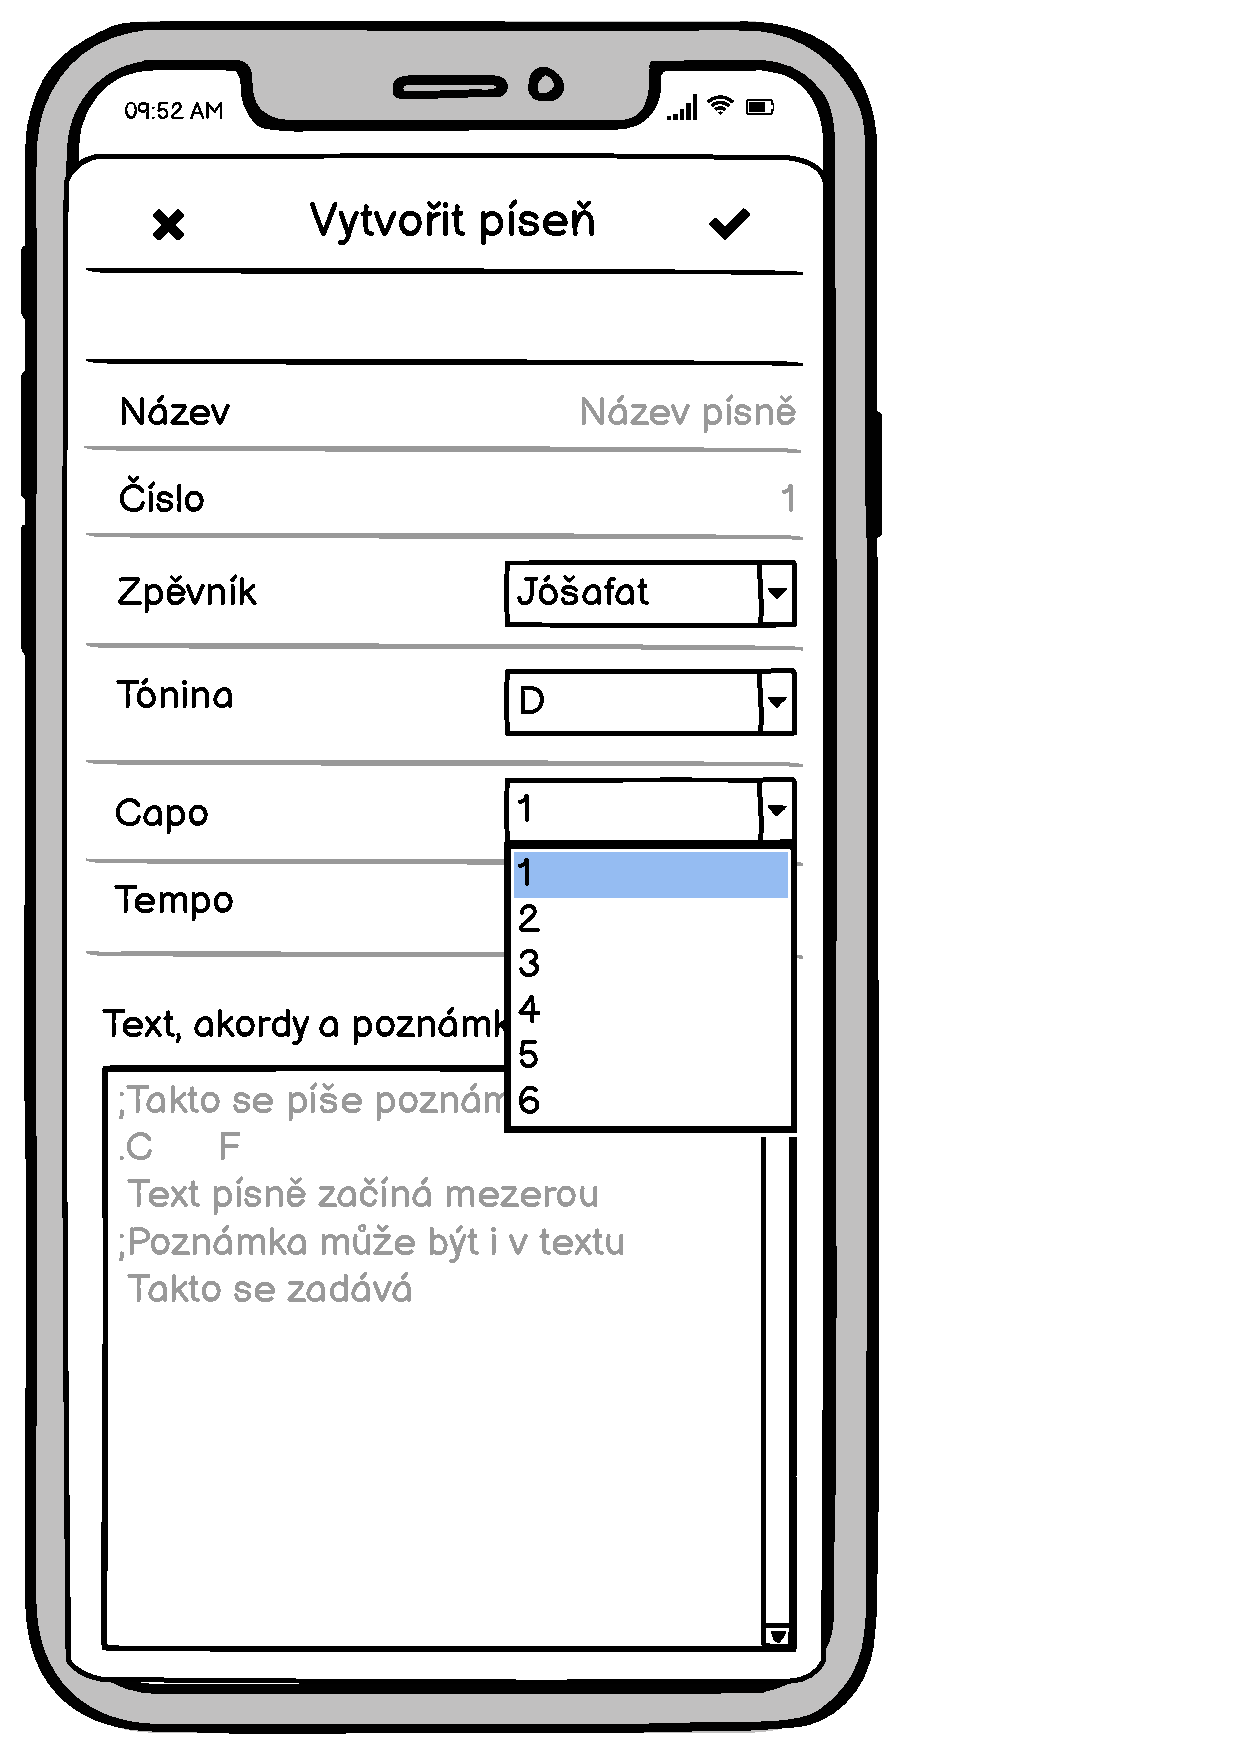
\includegraphics[width=0.49\textwidth]{images/B-navrh-ui/B-5-nova-pisen.pdf}
    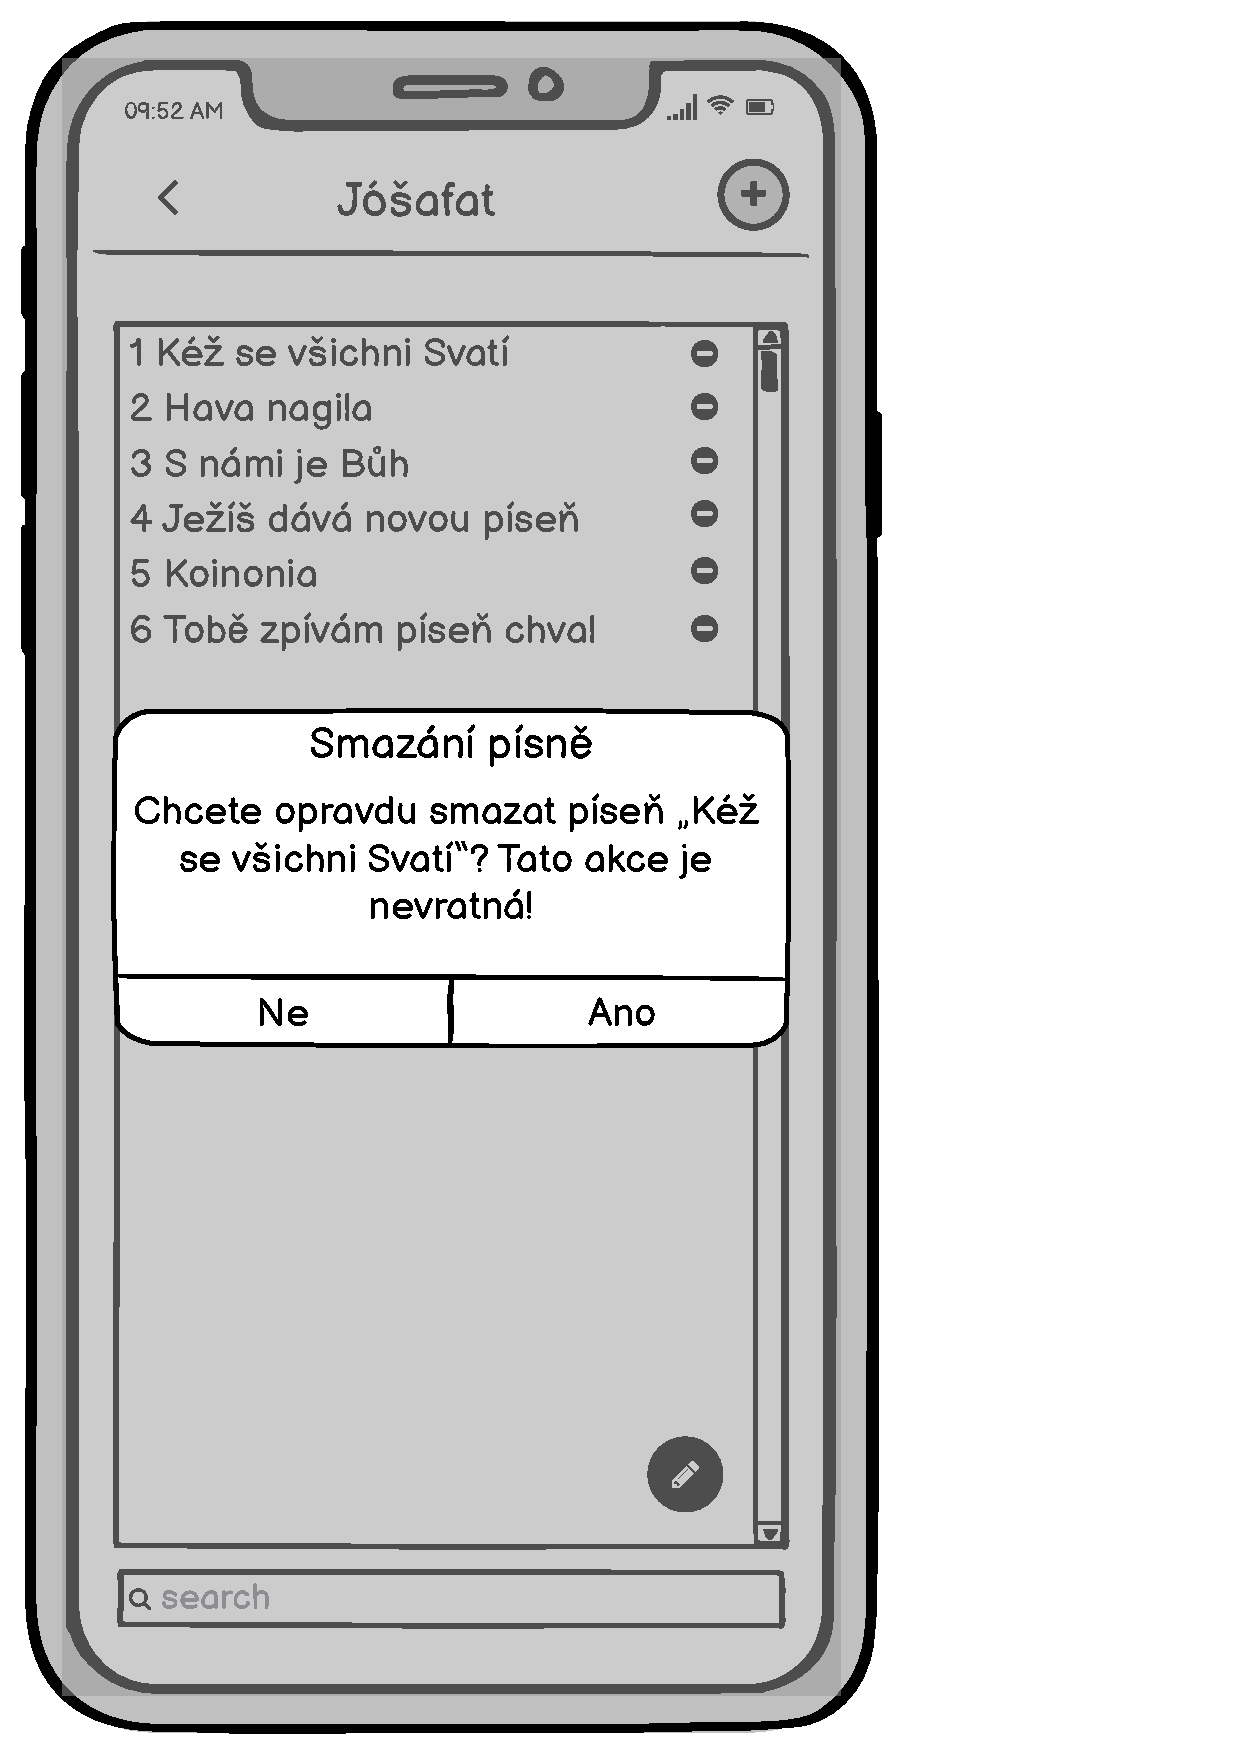
\includegraphics[width=0.49\textwidth]{images/B-navrh-ui/B-5-smazat-pisen.pdf}
    \caption{Vytvoření/úprava písně a Smazání písně}
\end{figure}

% Stránka 6

\begin{figure}
    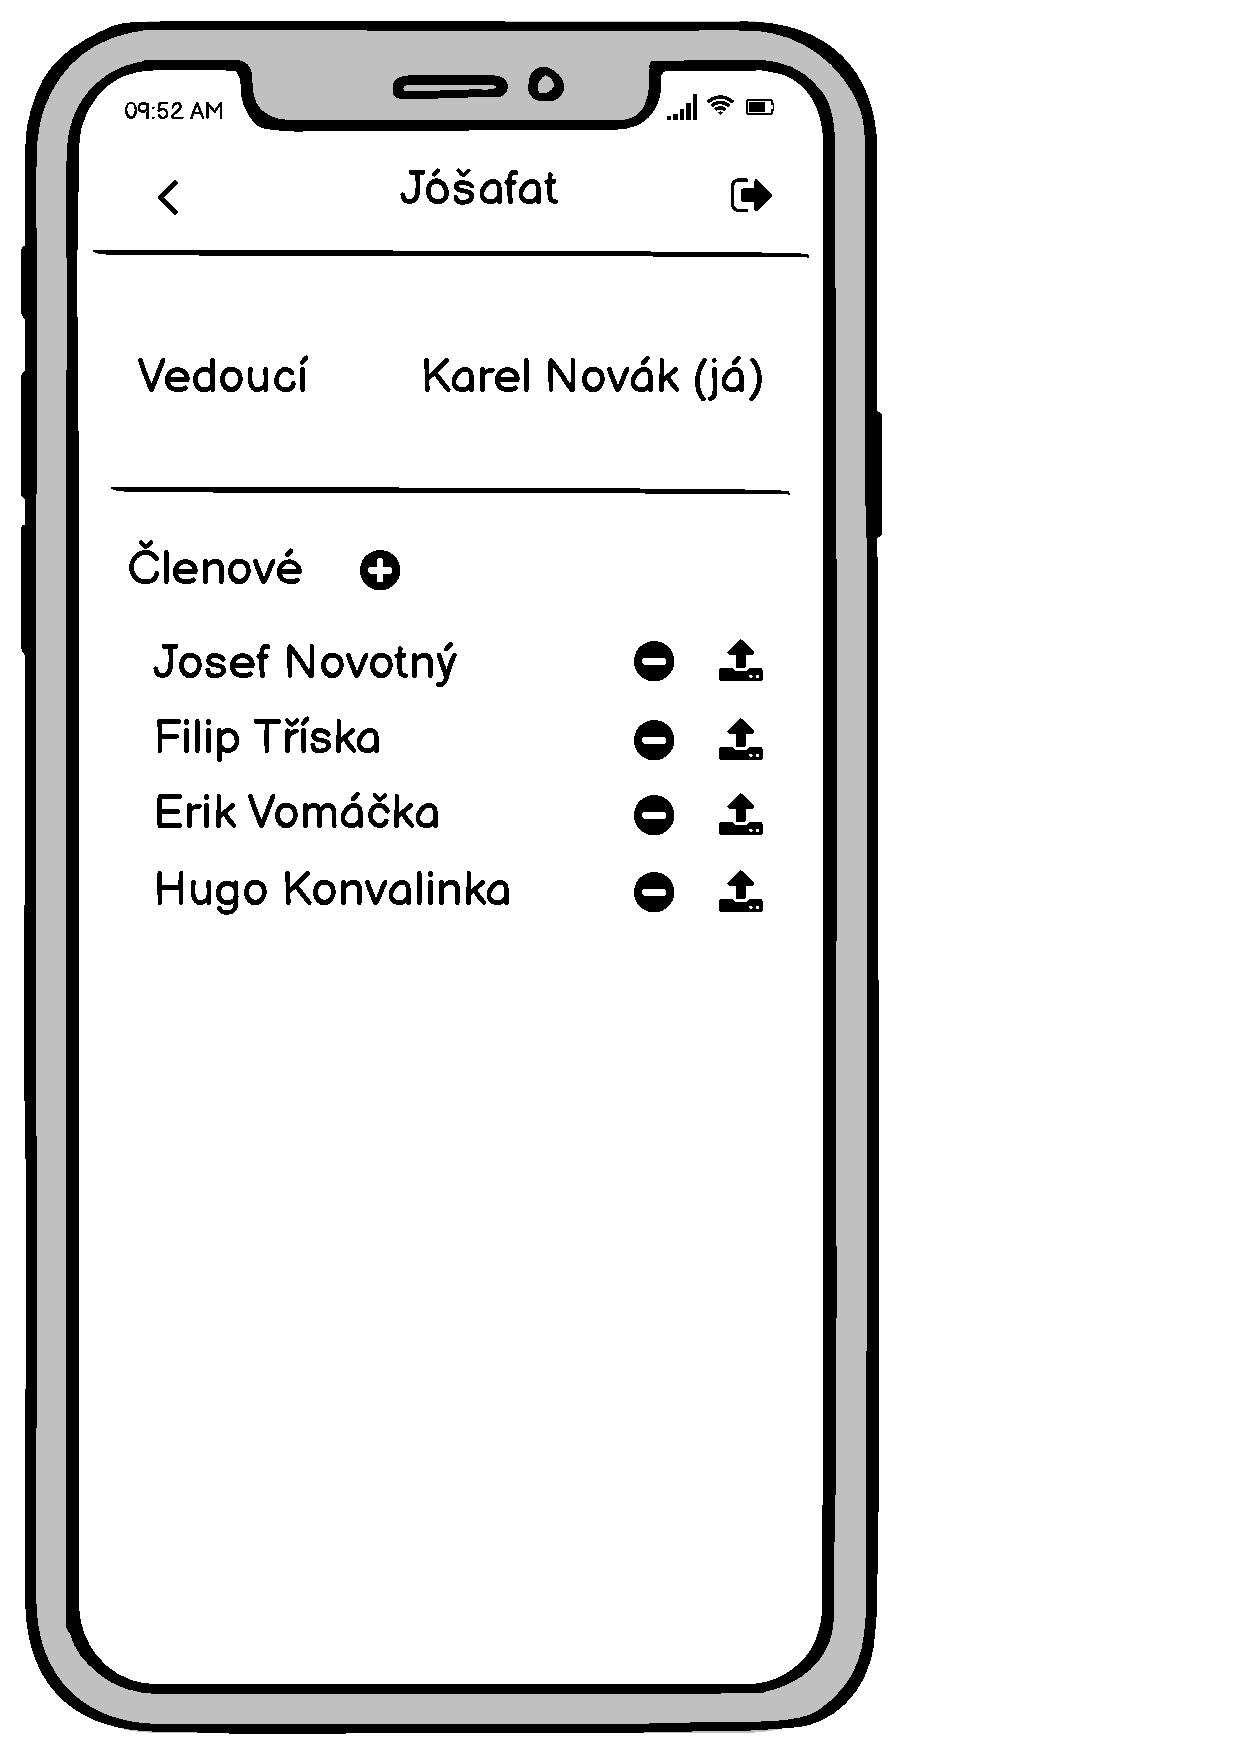
\includegraphics[width=0.49\textwidth]{images/B-navrh-ui/B-6-sprava-kapely.pdf}
    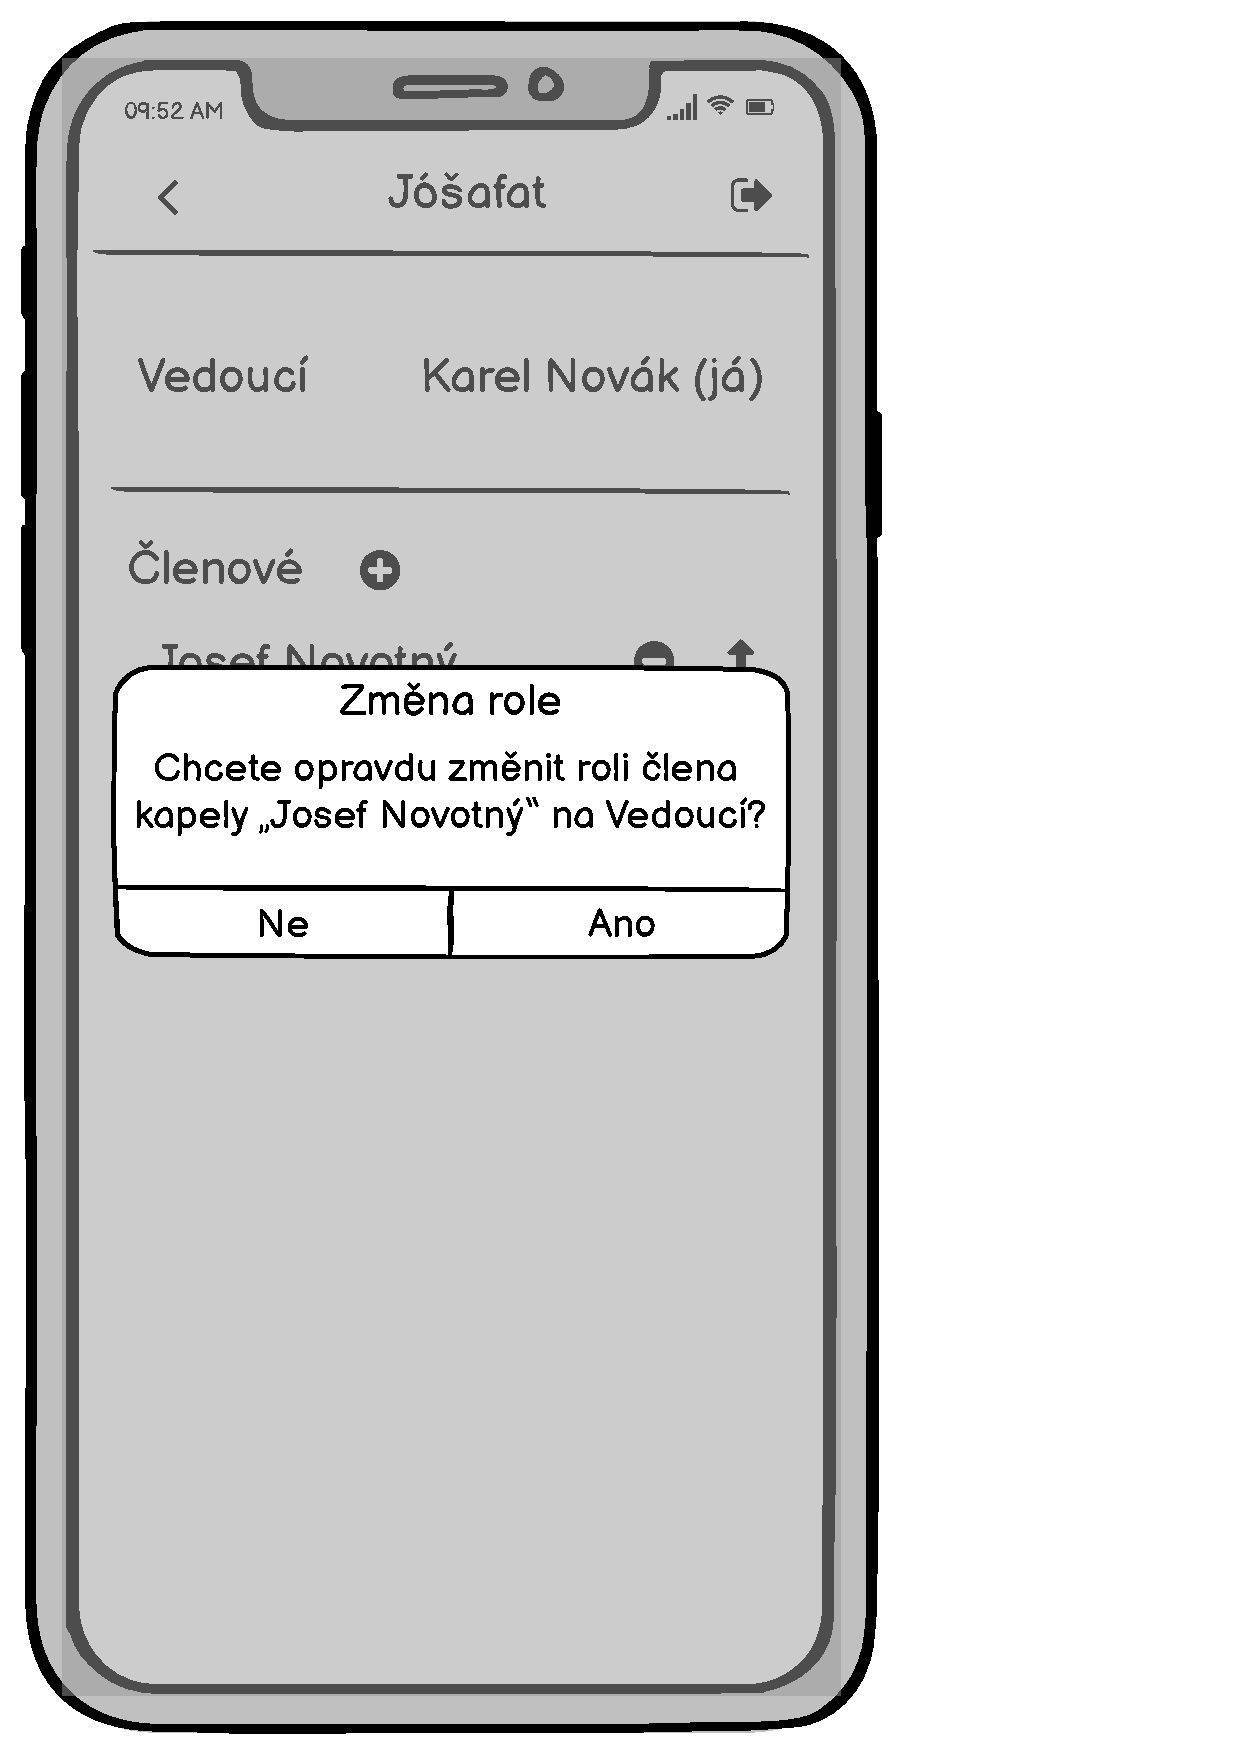
\includegraphics[width=0.49\textwidth]{images/B-navrh-ui/B-6-zmena-role.pdf}
    \caption{Správa kapely a dialog pro změnu role člena kapely}
\end{figure}

\chapter{Uživatelské rozhraní}

\begin{figure}[H]
    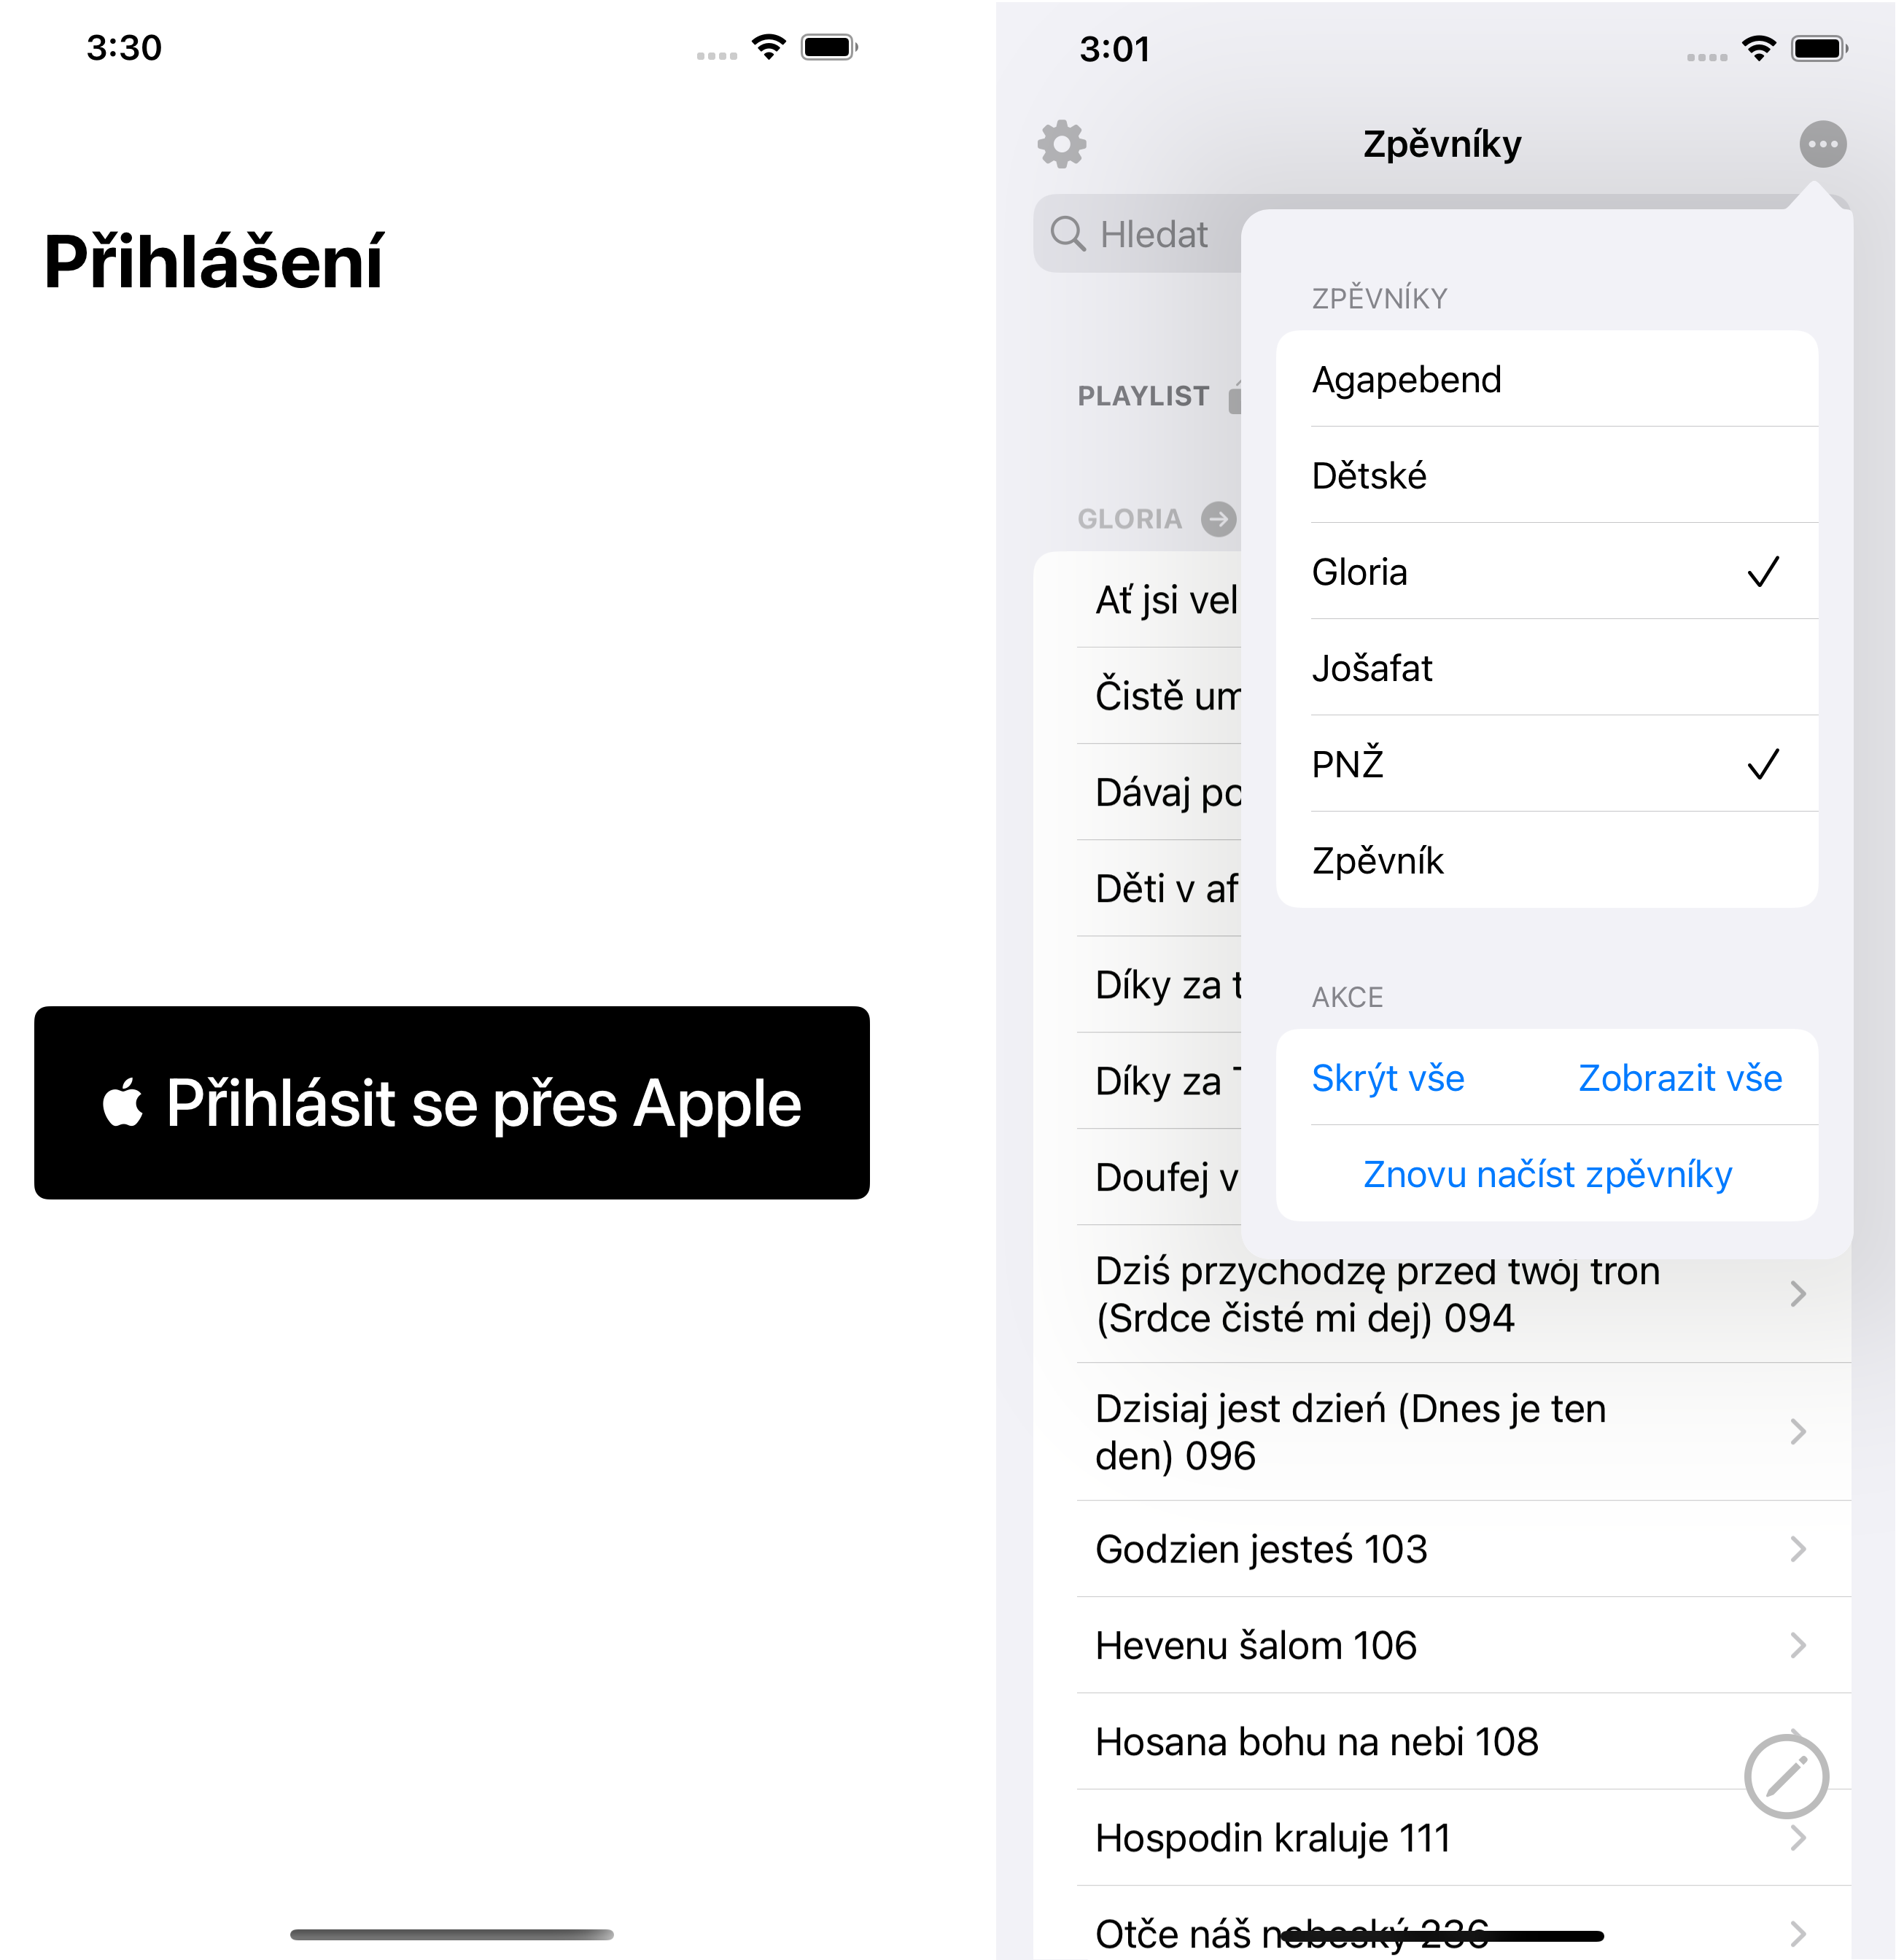
\includegraphics[width=0.9\textwidth]{images/C-ui/C-1-prihlaseni-seznam-zpevniku.png}
    \caption{Přihlášení a Seznam písní -- filtr zpěvníků}
\end{figure}

% Stránka 2

\begin{figure}
    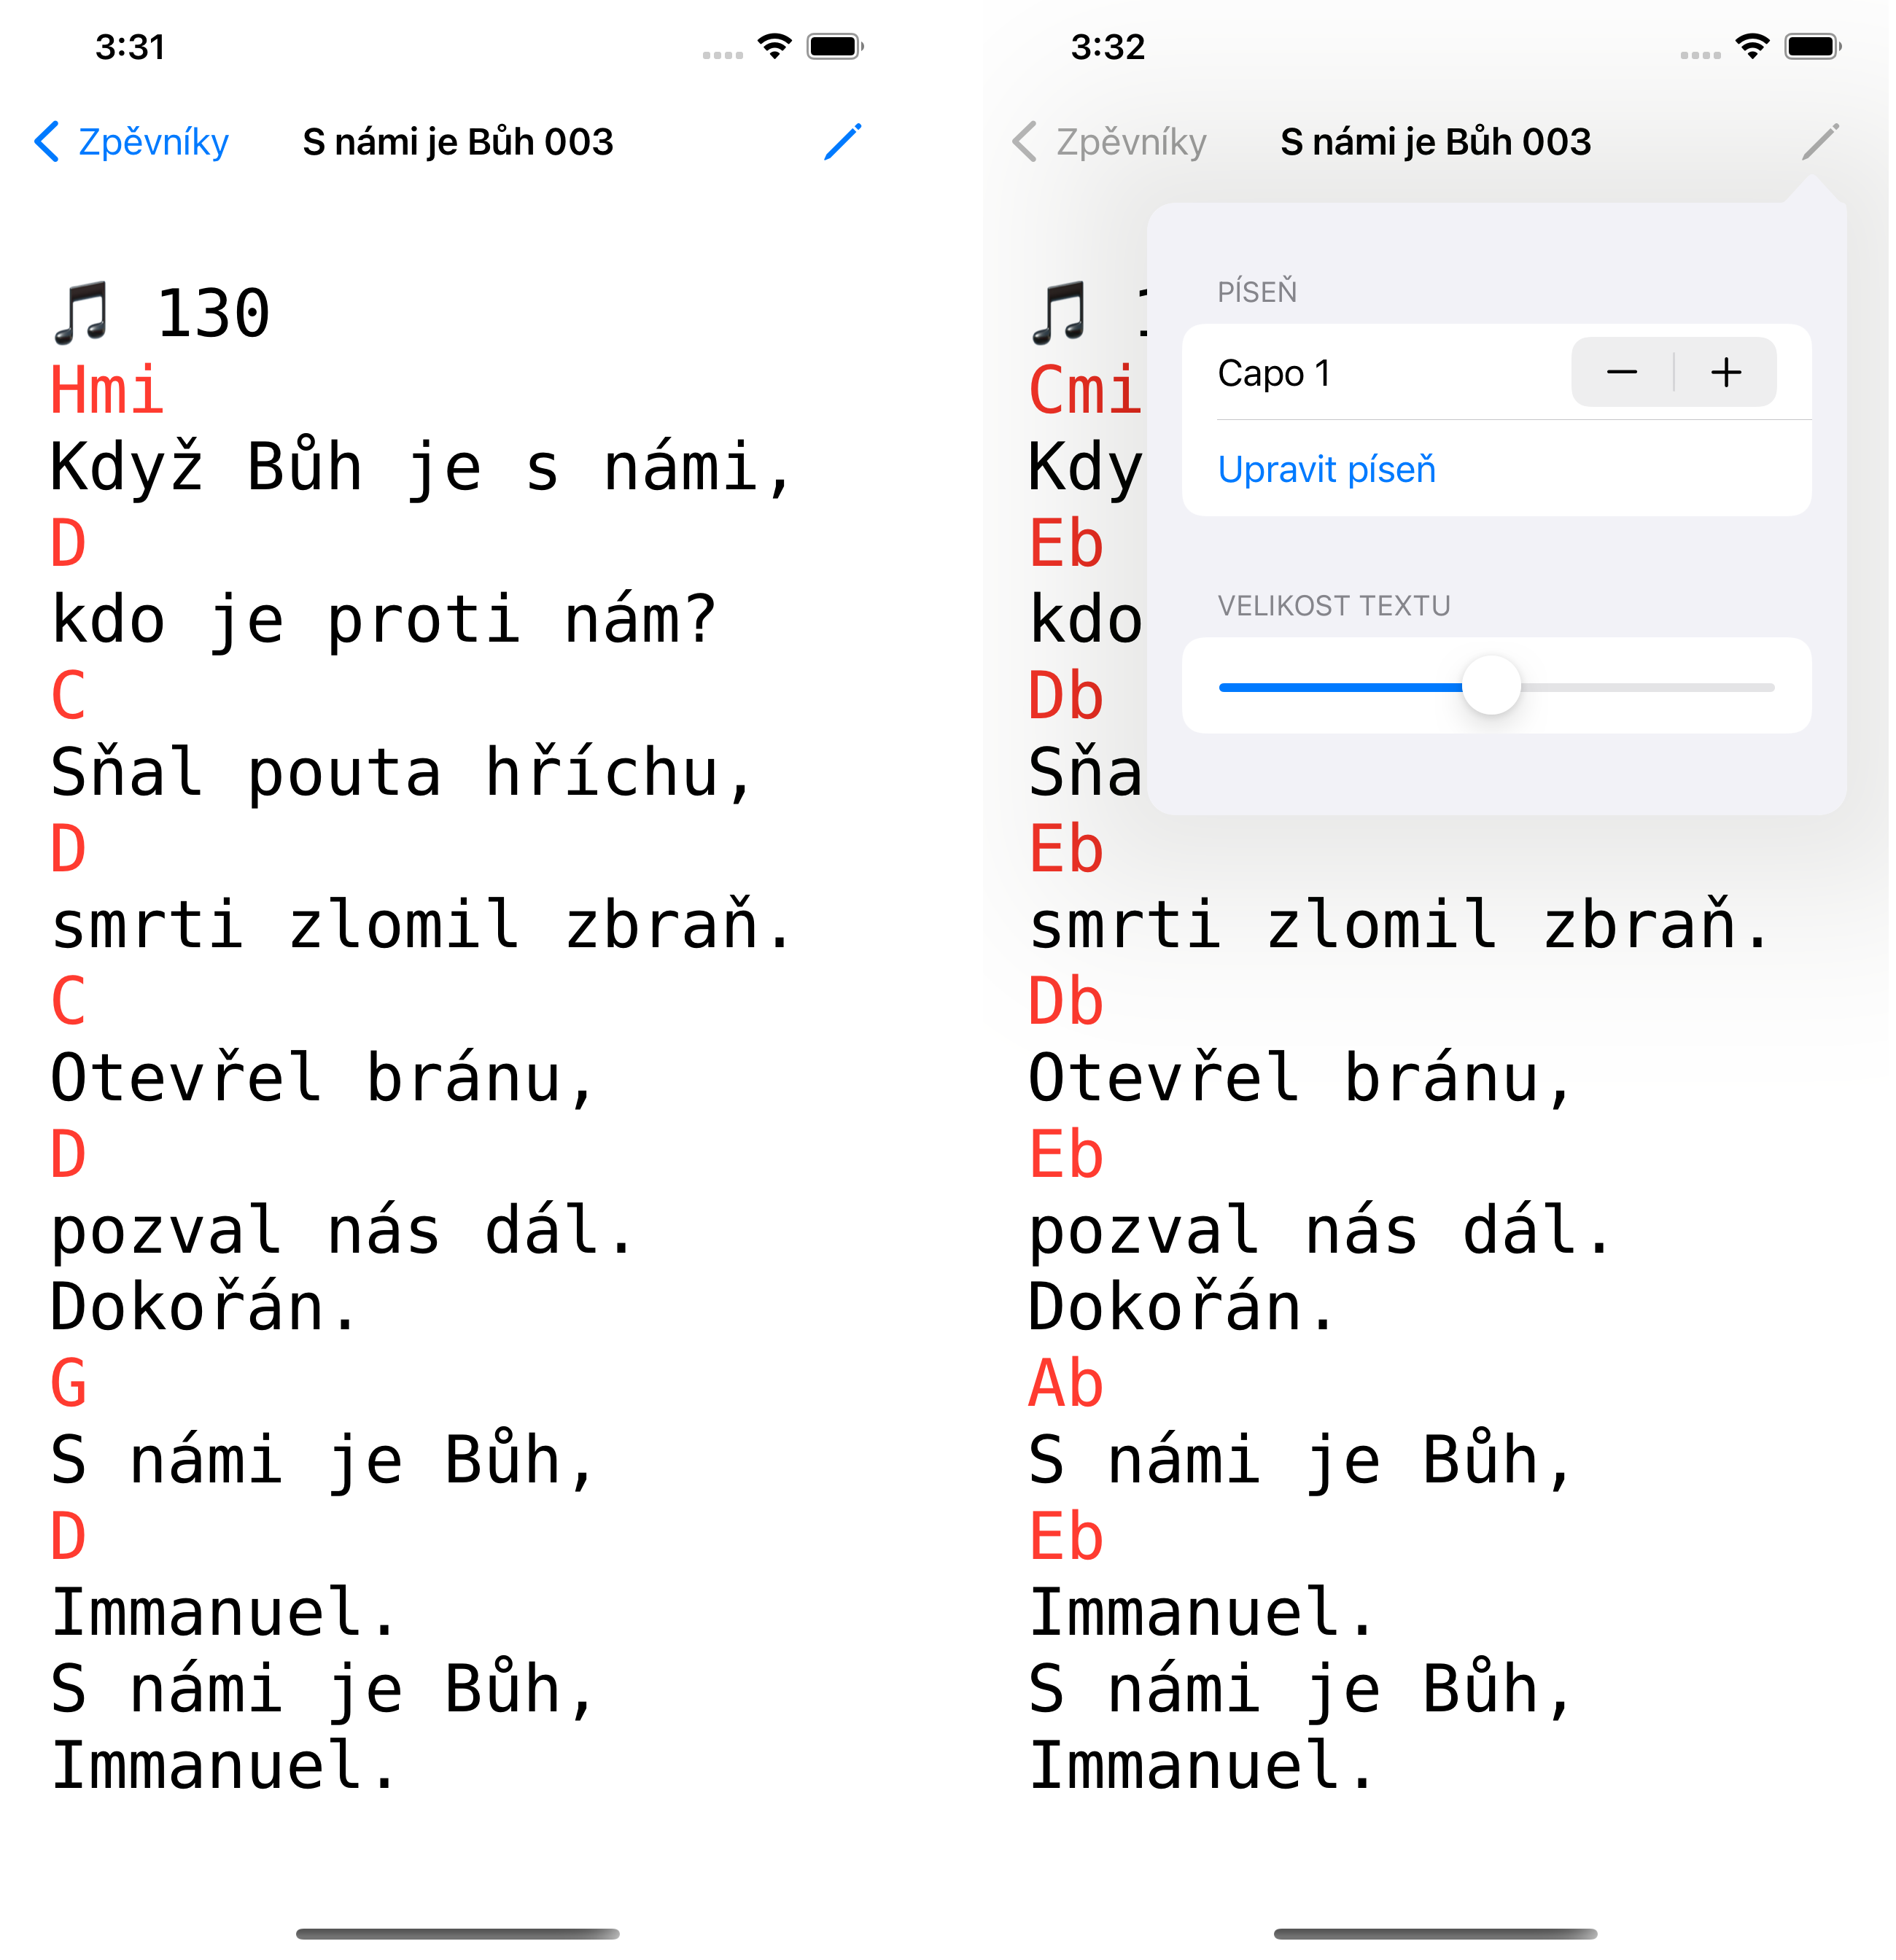
\includegraphics[width=\textwidth]{images/C-ui/C-2-detail-pisne.png}
    \caption{Detail písně a Nastavení písně}
\end{figure}

% Stránka 3

\begin{figure}
    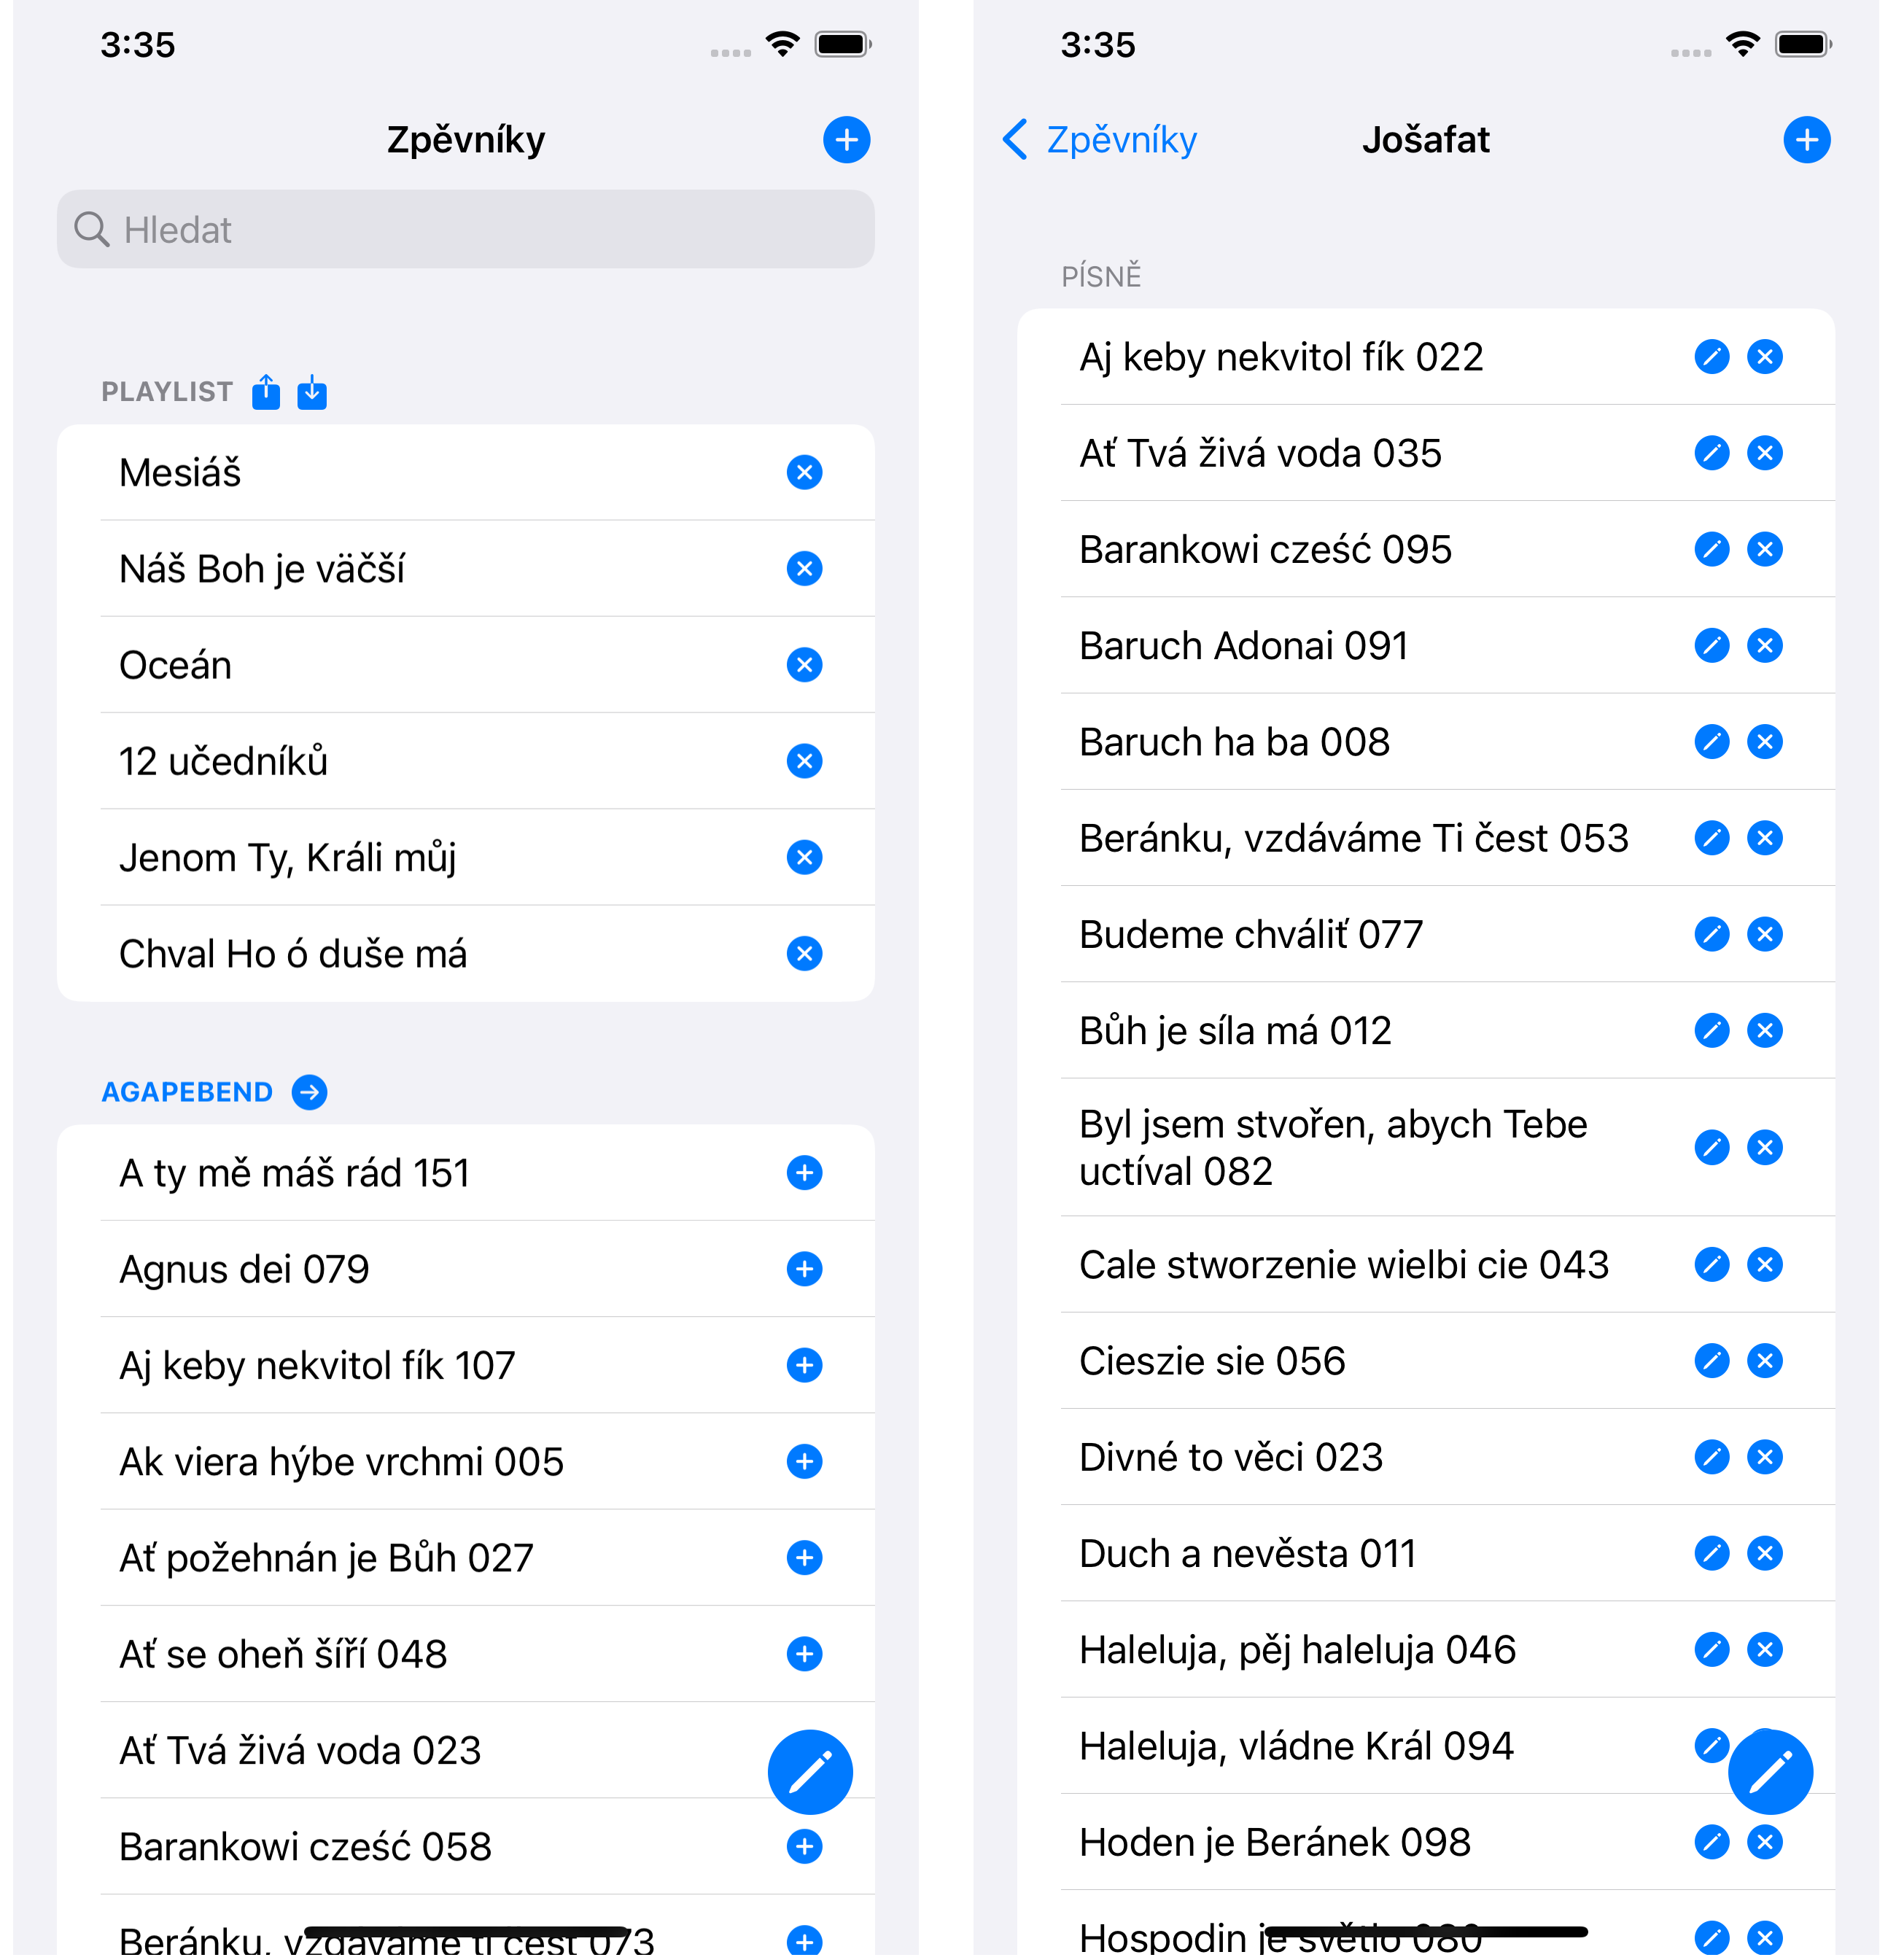
\includegraphics[width=\textwidth]{images/C-ui/C-3-sprava-zpevniku-pisni.png}
    \caption{Správa playlistů, zpěvníků a Správa písní ve zpěvníku}
\end{figure}

% Stránka 4

\begin{figure}
    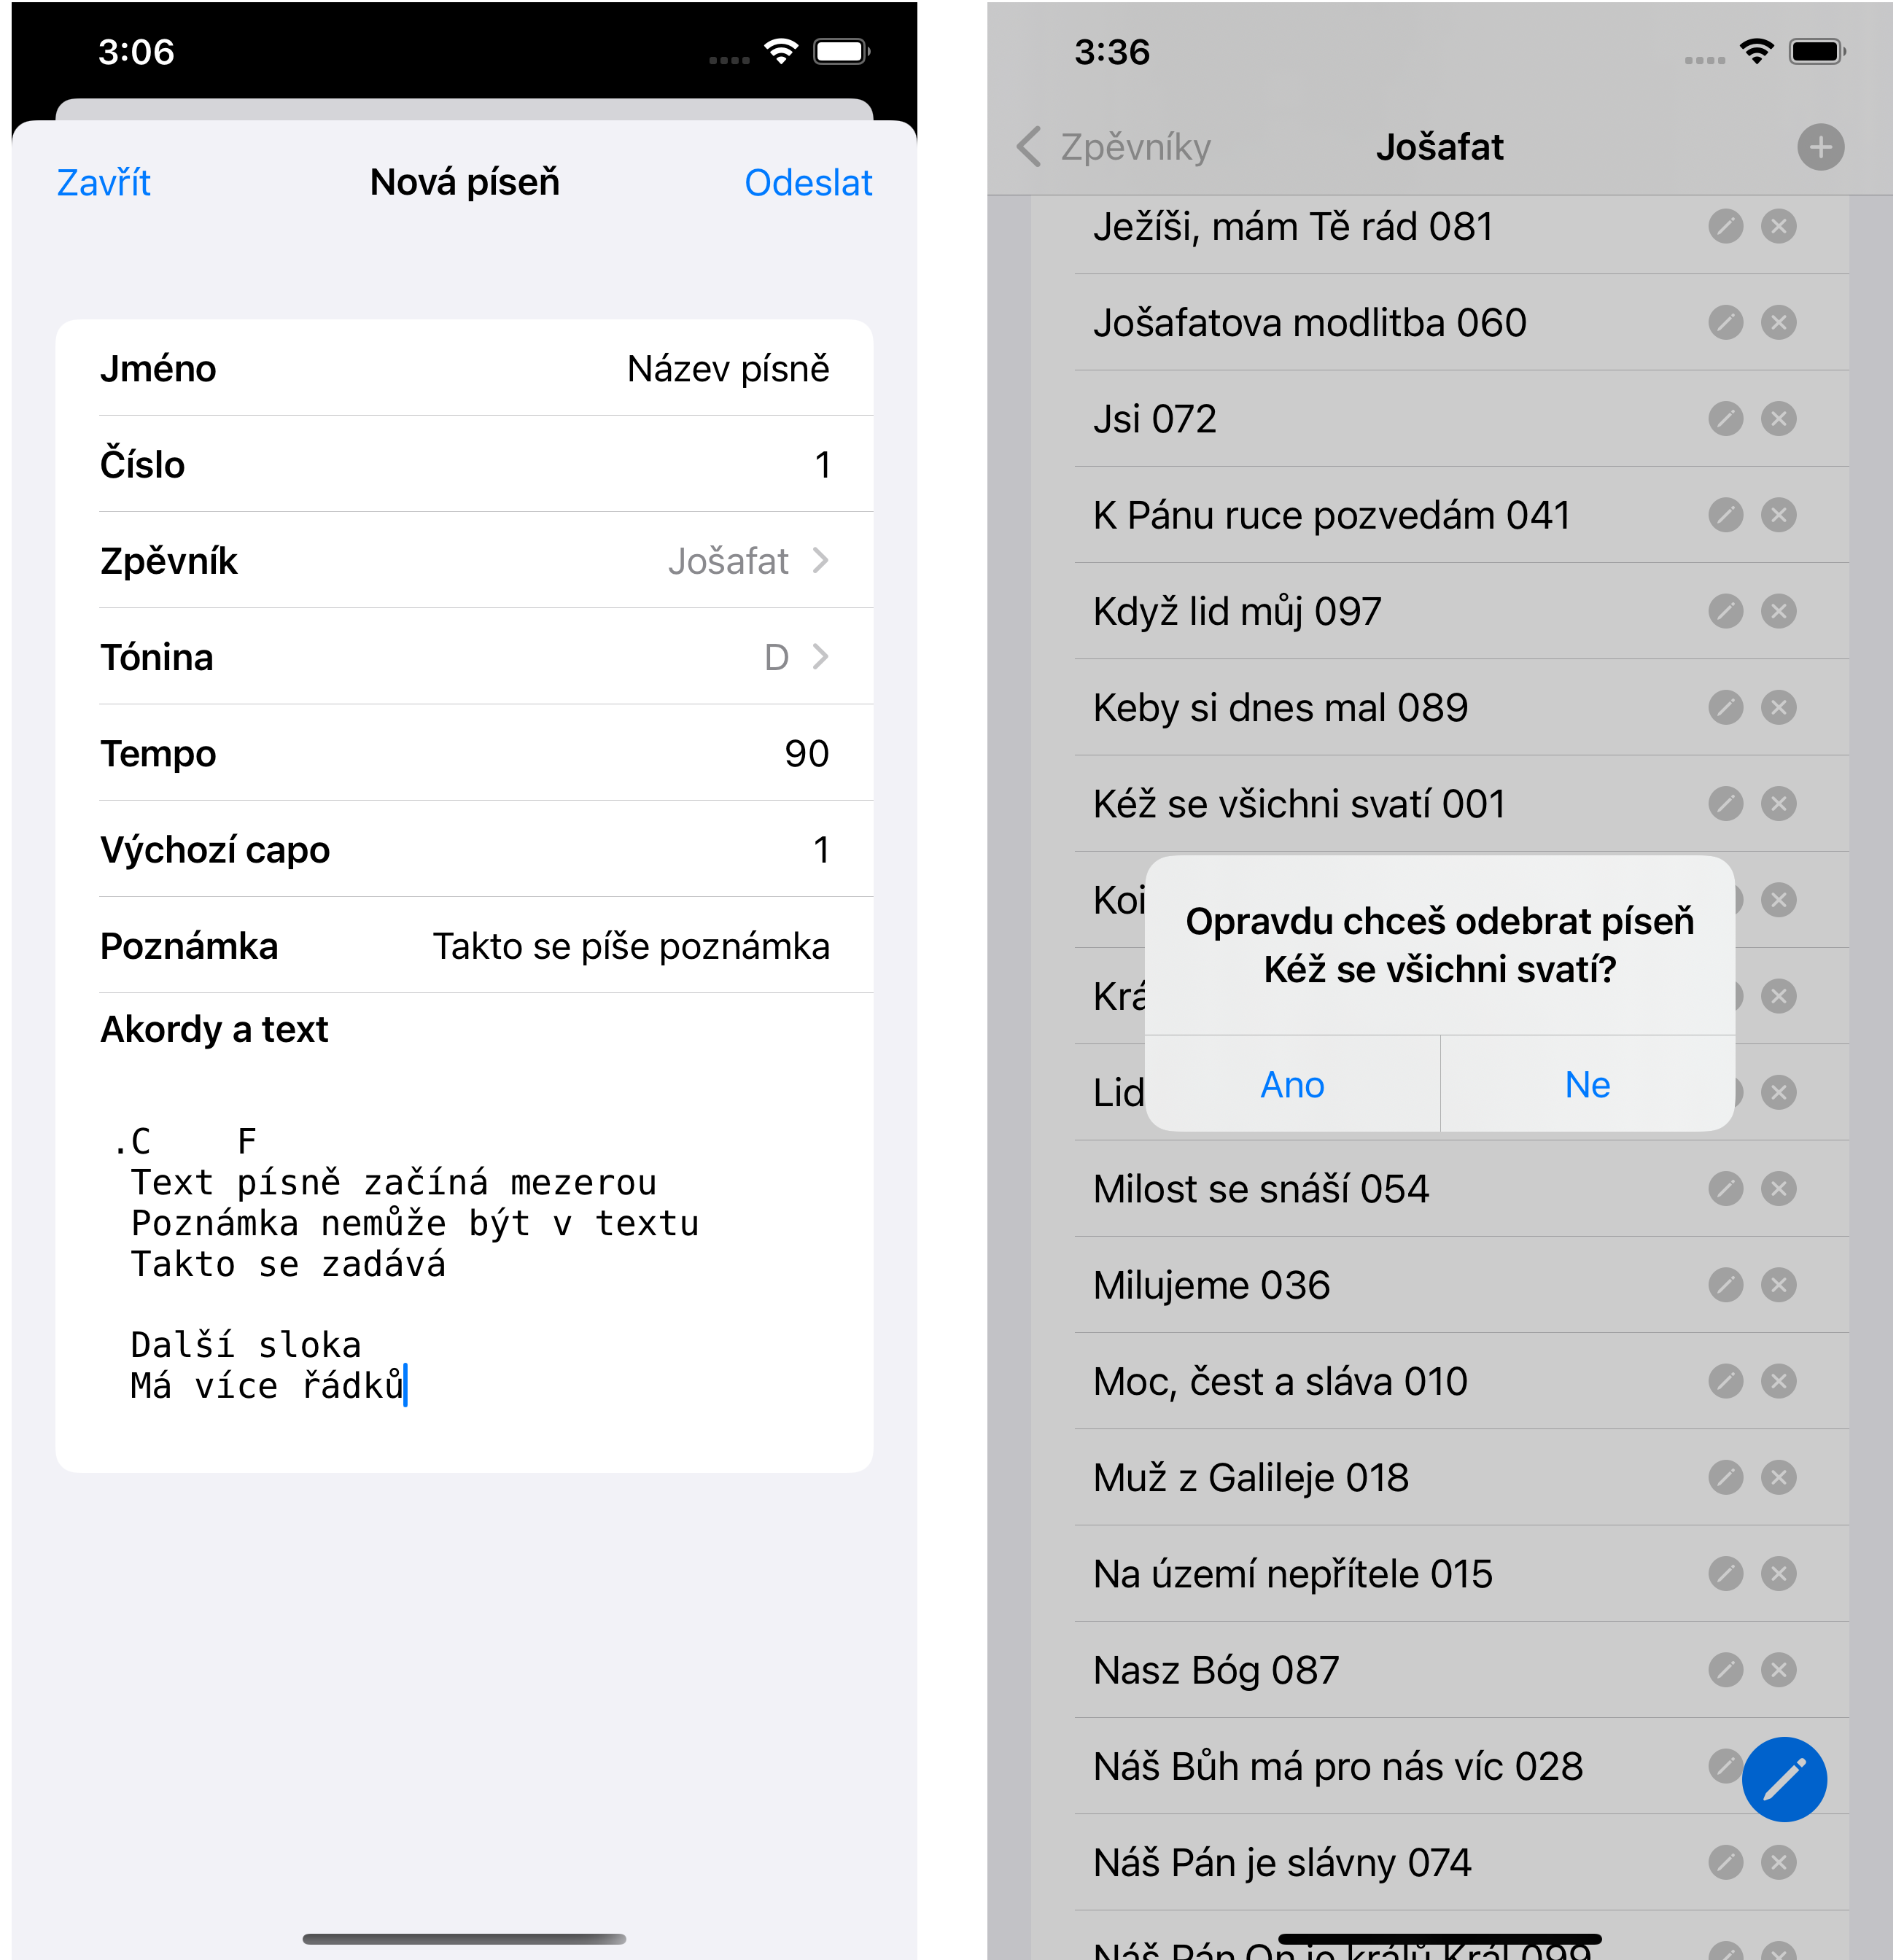
\includegraphics[width=\textwidth]{images/C-ui/C-4-nova-pisen-smazani-pisne.png}
    \caption{Vytvoření/úprava písně a Smazání písně}
\end{figure}

% Stránka 5

\begin{figure}
    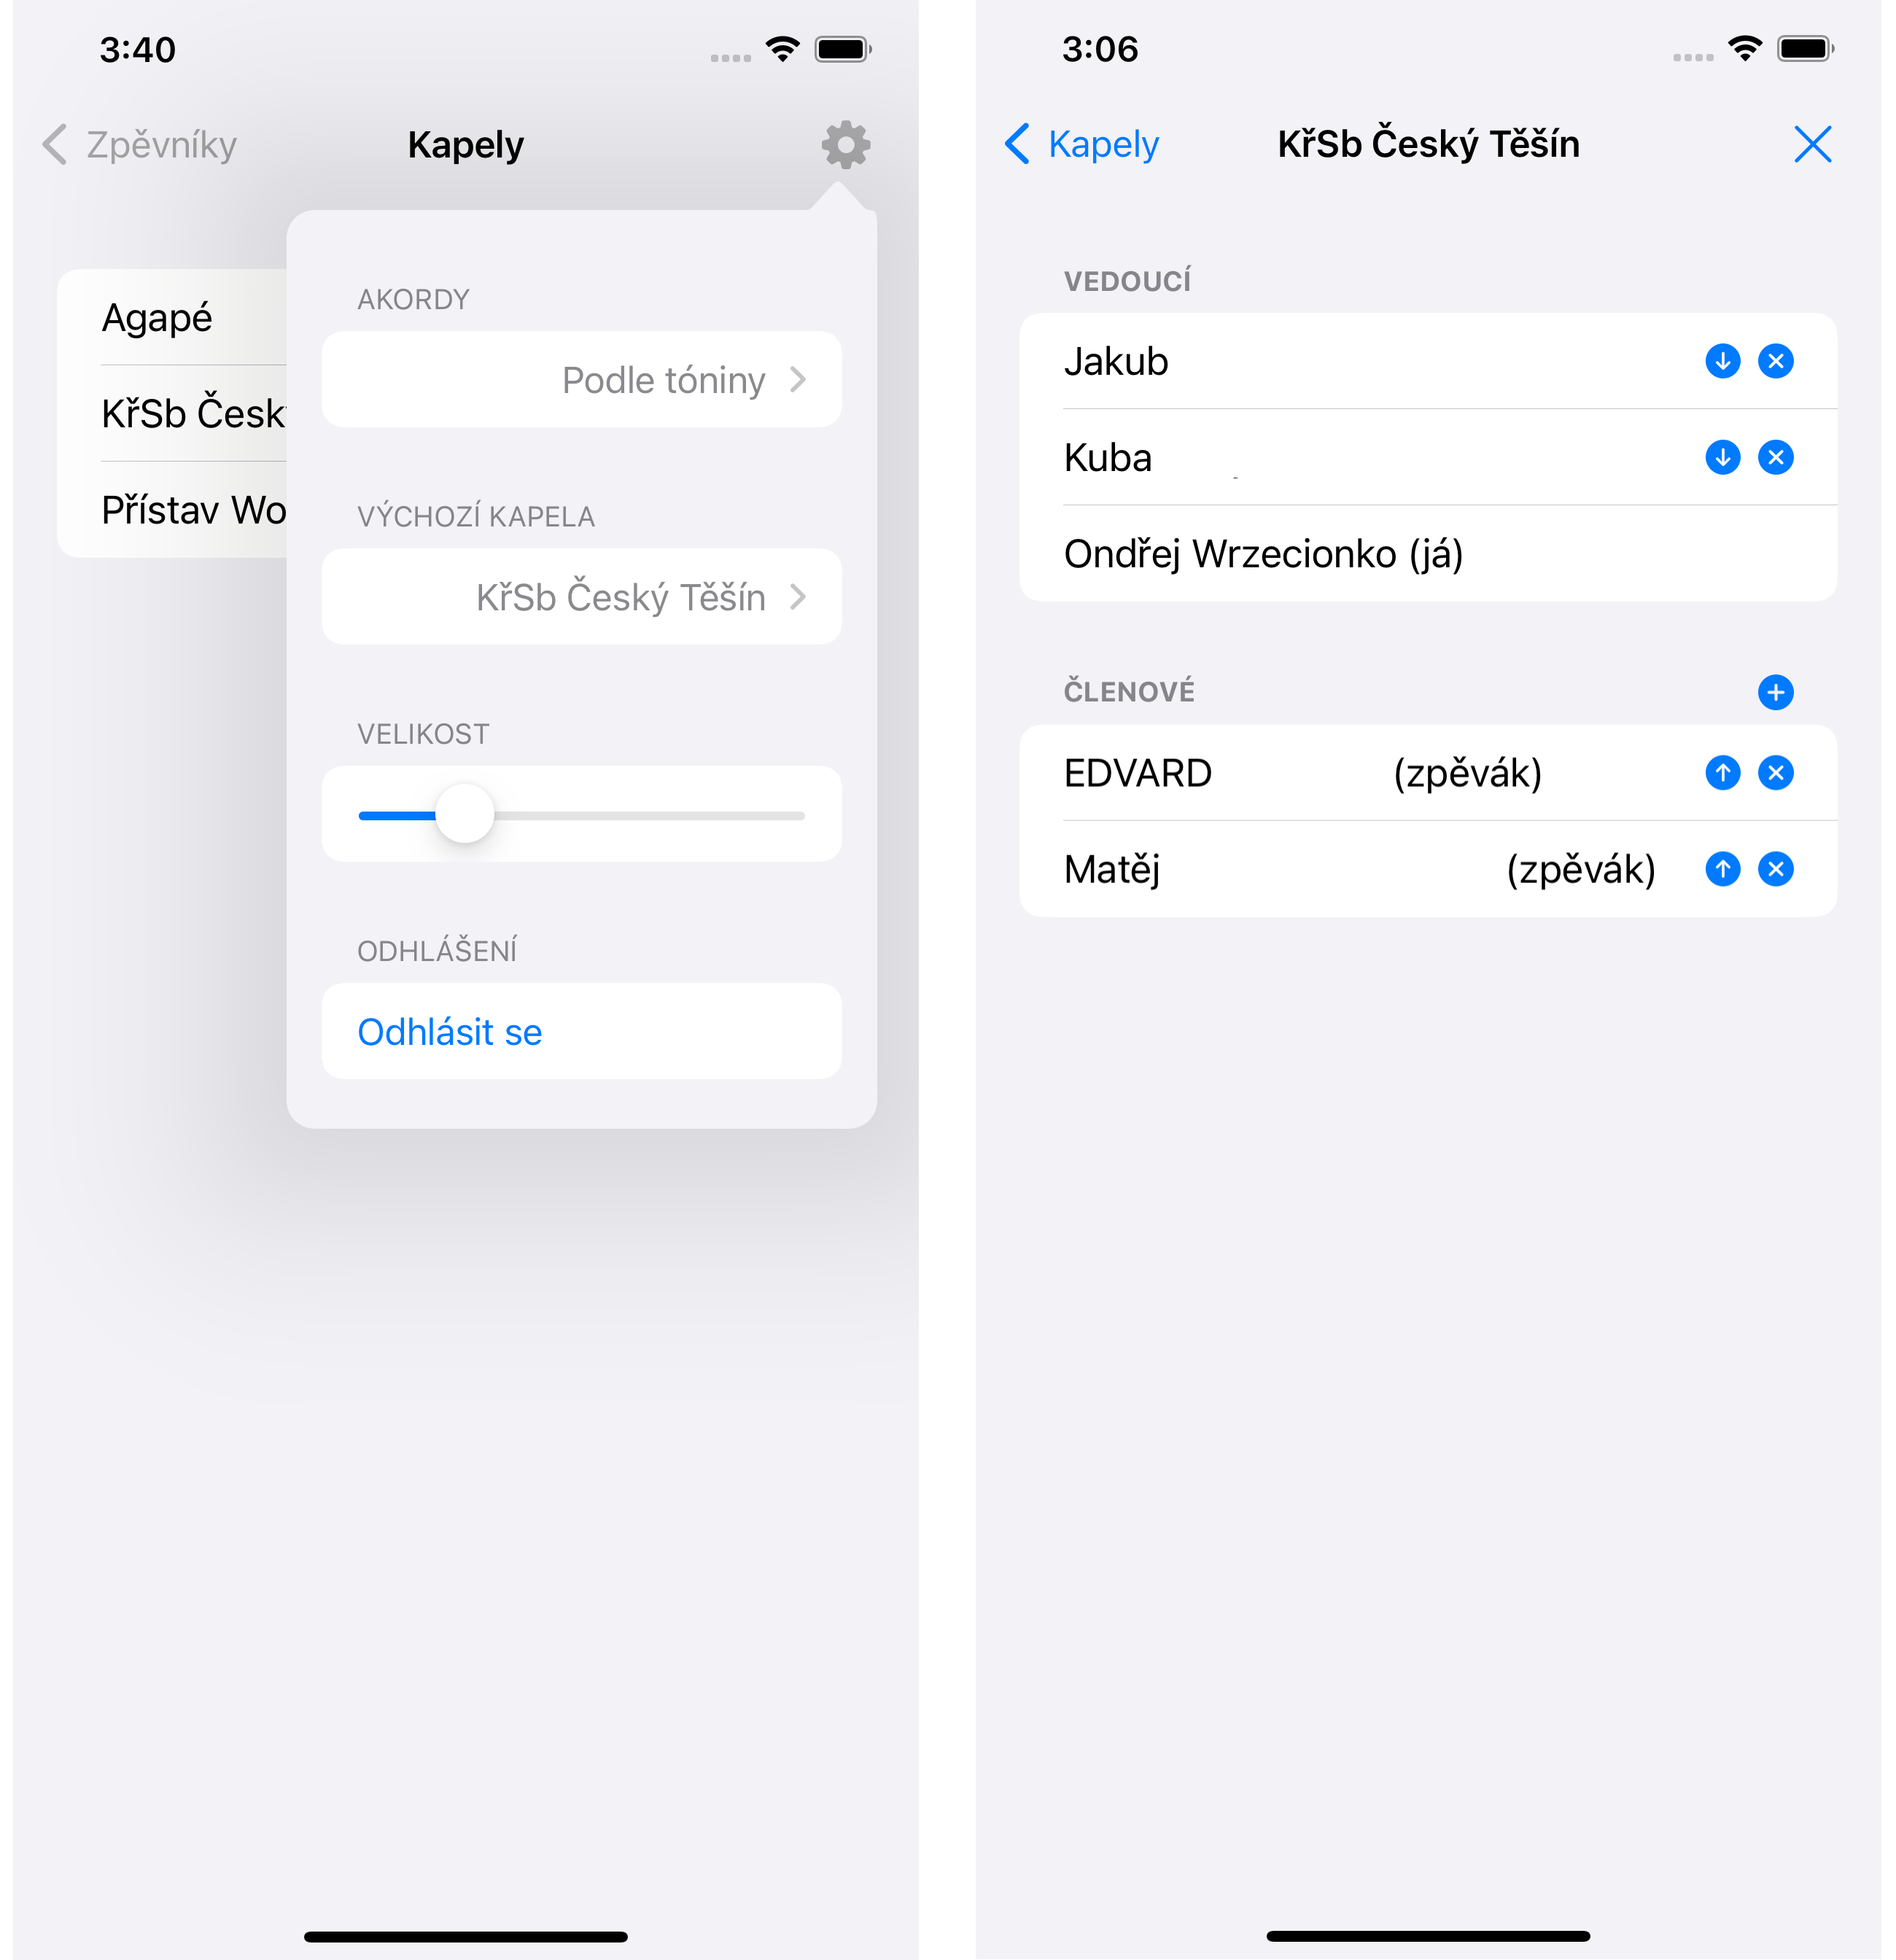
\includegraphics[width=\textwidth]{images/C-ui/C-5-nastaveni-aplikace-sprava-kapely.png}
    \caption{Nastavení aplikace a Správa kapely}
\end{figure}
